\documentclass[11pt, conference, letterpaper]{IEEEtran}

\usepackage{amsmath, amssymb, amsfonts}
\usepackage{graphicx}
\usepackage{algorithm}
\usepackage{algorithmic}
\usepackage{cite}
\usepackage{hyperref}
\usepackage{float}
\usepackage{dblfloatfix}
% \usepackage{appendix}
\usepackage{listings}
\usepackage{xcolor}  % Optional: For color syntax highlightings

\lstdefinestyle{python}{
    language=Python,
    basicstyle=\ttfamily\footnotesize,  % Choose font style and size
    keywordstyle=\color{blue},          % Color for keywords
    commentstyle=\color{green},         % Color for comments
    stringstyle=\color{red},            % Color for strings
    breaklines=true,                    % Line breaking
    numbers=left,                       % Line numbers on the left
    numberstyle=\tiny\color{gray},      % Style of the line numbers
    backgroundcolor=\color{white},      % Background color of the code box
    frame=single,                       % Add a frame around the code
    captionpos=b                        % Position of the caption (bottom)
}

% \renewcommand{\topfraction}{0.9}
% \renewcommand{\bottomfraction}{0.9}
% \renewcommand{\textfraction}{0.1}
% \renewcommand{\floatpagefraction}{0.9}

\begin{document}

\title{Kanade-Lucas-Tomasi (KLT) Feature Tracker: Theory, Implementations, and Performance Analysis}

\author{
\IEEEauthorblockN{Weston Scott}
\IEEEauthorblockA{Department of Electrical and Computer Engineering\\ University of Arizona\\ Email: scottwj@arizona.edu}
}

\maketitle

\thispagestyle{plain}  % Page number on the first page
\pagestyle{plain} 

\begin{abstract}
This paper presents an implementation and analysis of the Kanade-Lucas-Tomasi (KLT) feature tracker. The KLT algorithm is widely used in computer vision for tracking features across video frames due to its computational efficiency and accuracy. This report provides a theoretical background of the KLT algorithm, focusing on Shi-Tomasi corner detection and Lucas-Kanade optical flow. The practical implementation is discussed, and the algorithm's performance is evaluated under various scenarios and parameter settings. A comprehensive quantitative performance analysis is provided, assessing accuracy, robustness, and computation time.
\end{abstract}

\section{Introduction}
The Kanade-Lucas-Tomasi (KLT) feature tracker is a cornerstone in computer vision applications, particularly in motion analysis, object tracking, and video stabilization. By leveraging local feature properties, the KLT algorithm tracks features between consecutive video frames efficiently. This report focuses on implementing the KLT tracker and evaluating its performance under various scenarios and parameter settings. Additionally, challenges encountered during the implementation and proposed solutions are discussed.

\section{Theoretical Background}
The KLT feature tracker combines two key components: Shi-Tomasi corner detection for identifying robust features and Lucas-Kanade optical flow for tracking those features across frames. This section provides a detailed explanation of both components.

%%%%%%%%%%%%%%%%%%%%%%%%%%%%%%%%%%%%%%%%%%%%%%%%%%%%%%%%%

\subsection{Shi-Tomasi Corner Detection}
The Shi-Tomasi corner detector identifies strong features (corners) by analyzing the local image structure. The method is based on the observation that corners are regions where the intensity gradient has significant variation in multiple directions.

\subsubsection{Structure Tensor}
The structure tensor, also known as the second-moment matrix, is computed for a small window \(W\) around each pixel:
\begin{equation}
M = \begin{bmatrix}
\sum_W I_x^2 & \sum_W I_x I_y \\
\sum_W I_x I_y & \sum_W I_y^2
\end{bmatrix},
\end{equation}
where \(I_x\) and \(I_y\) are the spatial intensity gradients in the \(x\)- and \(y\)-directions, respectively.

The elements of the structure tensor have the following interpretations:
\begin{itemize}
    \item \(I_{xx} = \sum_W I_x^2\): The squared gradient in the \(x\)-direction, \((\frac{\partial I}{\partial x})^2\), which measures changes in intensity along the horizontal axis.
    \item \(I_{yy} = \sum_W I_y^2\): The squared gradient in the \(y\)-direction, \((\frac{\partial I}{\partial y})^2\), which measures changes in intensity along the vertical axis.
    \item \(I_{xy} = \sum_W I_x I_y\): The product of gradients in the \(x\)- and \(y\)-directions, \((\frac{\partial I}{\partial x})(\frac{\partial I}{\partial y})\), which captures the correlation between intensity changes along both axes.
\end{itemize}

These components characterize the local image structure and are used to evaluate intensity variations for identifying corners. 
\bigskip

\subsubsection{Gaussian Low Pass Filter}
After computing the components of the structure tensor, the image matrices Ixx, Iyy, and Ixy will be passed through a filter. A Gaussian low-pass filter alters the frequency content of a signal by attenuating high-frequency components. The parameter \(\sigma\) directly impacts the filter's behavior in both the spatial and frequency domains.

The Gaussian filter is defined in the spatial domain by the equation:
\[
G(x, y) = \frac{1}{2\pi\sigma^2} \exp\left(-\frac{x^2 + y^2}{2\sigma^2}\right),
\]
where:
\begin{itemize}
    \item \(x\) and \(y\) are the spatial coordinates relative to the center of the filter.
    \item \(\sigma\) is the standard deviation, controlling the extent of smoothing.
\end{itemize}

The kernel for a Gaussian filter can be discretely approximated in a computational implementation using:
\[
G[i, j] = \exp\left(-\frac{(i - \text{center}_x)^2 + (j - \text{center}_y)^2}{2\sigma^2}\right),
\]
where:
\begin{itemize}
    \item \(i\) and \(j\) are the discrete coordinates of the kernel.
    \item \(\text{center}_x\) and \(\text{center}_y\) are the indices of the kernel center.
    \item the resulting values are normalized such that their sum equals 1.
\end{itemize}

In the frequency domain, the Gaussian filter has the form:
\[
H(u, v) = \exp\left(-2\pi^2\sigma^2 (u^2 + v^2)\right),
\]
where \(u\) and \(v\) are the frequency domain coordinates. The filter attenuates high-frequency components by reducing their amplitudes, while retaining low-frequency components.


\begin{itemize}
    \item \textbf{Small \(\sigma\):}
    \begin{itemize}
        \item Retains high-frequency components, preserving edges and fine details.
        \item Narrow impulse response in the spatial domain (localized smoothing).
        \item Steep roll-off in the frequency domain, providing selective frequency attenuation.
        \item Minimal blurring, making it suitable for applications requiring detail preservation.
        \item Applications: Edge detection preprocessing, noise smoothing while retaining details.
    \end{itemize}
    \item \textbf{Large \(\sigma\):}
    \begin{itemize}
        \item Suppresses high-frequency components, leading to significant smoothing.
        \item Broad impulse response in the spatial domain (global smoothing).
        \item Gentle roll-off in the frequency domain, causing a more gradual transition.
        \item Effective for noise reduction but causes blurring of edges and fine details.
        \item Applications: Strong noise suppression, down-sampling, or coarse feature extraction
    \end{itemize}
\end{itemize}

% \begin{table}[]
%     \centering
%     \begin{tabular}{@{}lcc@{}}
%         \toprule
%         \textbf{Parameter} & \textbf{Small \(\sigma\)} & \textbf{Large \(\sigma\)} \\ \midrule
%         Frequency Cutoff   & High (retains more high frequencies) & Low (removes more high frequencies) \\
%         Bandwidth          & Wide (less aggressive filtering)     & Narrow (more aggressive filtering) \\
%         Roll-off           & Steep (sharp transitions)            & Gentle (broad transitions) \\
%         Spatial Smoothing  & Minimal (localized)                  & Strong (global) \\
%         SNR Improvement    & Limited                              & Significant \\
%         Edge Preservation  & Good (details retained)              & Poor (details blurred) \\ \bottomrule
%     \end{tabular}
%     \caption{Effects of \(\sigma\) on Gaussian Low-Pass Filtering}
% \end{table}

\bigskip


\subsubsection{Corner Criterion}
The quality of a corner is evaluated using the eigenvalues \(\lambda_1\) and \(\lambda_2\) of \(M\). The Shi-Tomasi criterion simplifies the selection process by considering the smaller eigenvalue:
\begin{equation}
R = \min(\lambda_1, \lambda_2).
\end{equation}
A pixel is classified as a corner if \(R > \text{threshold}\).
\bigskip

\subsubsection{Feature Selection}
To ensure spatial diversity in detected features, a minimum distance constraint is applied between selected corners. This reduces redundancy and improves feature quality.
\bigskip

%%%%%%%%%%%%%%%%%%%%%%%%%%%%%%%%%%%%%%%%%%%%%%%%%%%%%%%%%

\subsection{Lucas-Kanade Optical Flow}
Lucas-Kanade optical flow is a local method for tracking the movement of features between consecutive frames. It assumes that the intensity of a feature remains constant as it moves and that the motion within a small neighborhood is approximately constant. Shi-Tomasi corners are foundational for this algorithm, since the corners that are detected are what the Optical Flow equations are working with.

\subsubsection{Optical Flow Constraint Equation}
The optical flow constraint assumes that the intensity of a pixel remains unchanged:
\begin{equation}
I(x, y, t) = I(x + \Delta x, y + \Delta y, t + \Delta t).
\end{equation}
Expanding this equation using a Taylor series and ignoring higher-order terms leads to:
\begin{equation}
I_x u + I_y v + I_t = 0,
\end{equation}
where \(I_x\) and \(I_y\) are spatial intensity gradients, \(I_t\) is the temporal gradient, and \((u, v)\) is the flow vector.
\bigskip

\subsubsection{Weighted Least-Squares Solution}
The motion vector \((u, v)\) is determined by minimizing the weighted sum of squared errors in a window \(W\):
\begin{equation}
\begin{bmatrix}
\sum_W I_x^2 & \sum_W I_x I_y \\
\sum_W I_x I_y & \sum_W I_y^2
\end{bmatrix}
\begin{bmatrix}
u \\
v
\end{bmatrix}
=
\begin{bmatrix}
-\sum_W I_x I_t \\
-\sum_W I_y I_t
\end{bmatrix}.
\end{equation}
\bigskip

\subsubsection{Pyramid Implementation}
To handle large displacements, the Lucas-Kanade method is implemented in a coarse-to-fine fashion using image pyramids. This involves tracking features at lower resolutions and refining them at higher resolutions.

%%%%%%%%%%%%%%%%%%%%%%%%%%%%%%%%%%%%%%%%%%%%%%%%%%%%%%%%%

\section{Implementation}
This section details the practical implementation of the Kanade-Lucas-Tomasi (KLT) feature tracker, focusing on Shi-Tomasi corner detection and Lucas-Kanade optical flow. The implementation was developed using Python, leveraging OpenCV for core functionalities and NumPy for custom optimizations.

\subsection{Shi-Tomasi Corner Detection}
The Shi-Tomasi corner detection algorithm was implemented to extract strong corners as the first step in the KLT feature tracker. The algorithm relies on the computation of the structure tensor and evaluates the minimum eigenvalue to determine corner quality.

\subsubsection{Key Parameters}
The following parameters were configured for the implementation:
\begin{itemize}
    \item \textbf{Max Corners:} Limits the number of corners detected, ensuring computational efficiency.
    \item \textbf{Quality Level:} A multiplier applied to the maximum eigenvalue to set a threshold for corner detection.
    \item \textbf{Minimum Distance:} Enforces spatial diversity by requiring a minimum distance between detected corners.
    \item \textbf{Kernel Size:} Specifies the size of the Sobel filter used for gradient calculation.
    \item \textbf{Gaussian Sigma:} Determines the standard deviation for Gaussian smoothing applied to the image.
\end{itemize}
\bigskip

\subsubsection{Implementation Details}
The algorithm uses OpenCV's \texttt{cv2.goodFeaturesToTrack} function for efficient corner detection as the baseline. Additionally, a custom implementation was developed for comparison, leveraging NumPy to compute the structure tensor and eigenvalues directly.
To enhance robustness, detected corners were refined using a scaled-down version of the image, ensuring that high-quality corners were retained while minimizing noise. 

Once the image was passed to the Shi-Tomasi routine (see code list \ref{lst:shi-tomasi}) routine with the other design parameters defined, the image would be converted to grayscale if not already, then the image would be convolved with a Sobel kernel in both the x and y directions to calculate Ix and Iy (see Figure \ref{fig:sobel_gradient}). 

Following these new convolved images, the components of the structure tensor (M) could be created, with Ixx showing the horizontal intensity change, Iyy the vertical intensity change, and Ixy the interaction between the directional intensity changes (see Figure \ref{fig:pre_gaussian_lpf}). These new images (matrices) are then sent through a low pass gaussian filter to reduces noise and minor variations, and overall smooth the image (see Figure \ref{fig:gaussian_lpf}). 

From there the minimum eigenvalues for each pixel are calculated (Shi-Tomasi score), and in tandem with the determinant of the structure tensor and a sensitivity response, quality corner candidates can be created for the image. These corner candidates are then sent sorted by strongest response, the sent through a density filter.

Writing the convolution algorithm in two dimensions was a challenge not due to the complexity of the problem, but due to the length of time is takes to have NumPy loop over the image with a kernel. After research and testing, the Numba library for Python was used to accelerate the code, allowing the convolutions to take place rapidly, allowing the development of the this part of the project to move forward (see code list \ref{lst:convolution}). The convolution routine that was written handles any kernel with image, as long as the kernel is smaller than the image itself. The image is zero padded always, to ensure that the spatial dimensions of the image is preserved, border pixel information isn't lost, and also aid in keeping the filters with a symmetric operation. The same convolution routine is used for both the Sobel Gradient (using a Sobel kernel, see code list \ref{lst:sobel-kernel}) and the Gaussian Low Pass Filter (using a Gaussian kernel, see code list \ref{lst:gaussian-kernel}) steps, making it generically usable my other routines written for various image operations and filters.

After the various image operations and computations were completed, it made sense to ensure that points were not overlapping. Typically using a max-suppression like algorithm could work for this, instead a filter was written to simply only allow points within a specified minimum pixel distance to pass through. This filter also ensured that no points along the edge of the image were detected. The minimum distance constraint was enforced to prevent clustering of corners in regions with high texture. See code list \ref{lst:corner_filter} for code implementation.

Work was started on introducing more image operations into the custom NumPy algorithm utilizing histogram equalization and other filter types such as a median filter or high pass filter. Basic code was developed to implement these ideas, but the time was not there to assess. These methods can be effective in helping to improve or degrade contrast in the image
\bigskip

\subsubsection{Visualization}
The detected corners were visualized by overlaying circles on the original frames. Each circle represented a corner, highlighting regions of interest identified by the algorithm. This visualization was instrumental in validating the accuracy and consistency of corner detection. Figures \ref{fig:shi_tomasi_results} and \ref{fig:shi_tomasi_results2} show side by side the pure NumPy (left) compared to the OpenCV.goodFeaturesToTrack (right) corner candidates instrumented with identical feature parameters. These images differ in sensitivity and number of allowable corners detectable.

Many hours were spent on plotting methods for grouping corner points after getting the corner detections to work. These methods include a simply distance grouping via pixel threshold, nearest neighbor look up based on a max distance, and k-means clustering. These methods are not shown in the resulting images, but the methods help to draw bounding boxes around areas of interest (more densely populated areas) especially when working through the design of the algorithm was underway.
\bigskip

\subsubsection{Performance Comparison}
A comparison between the custom implementation and OpenCV's functions revealed that the custom NumPy approach provided similar accuracy while allowing greater flexibility in parameter tuning. OpenCV's implementation, however, demonstrated superior computational efficiency, even after optimizing the code using advanced python libraries (Numba) to accelerate specific sections of code. For performance comparisons, a few metrics were employed to quantify the results between the NumPy and OpenCV implementations.

\begin{itemize}
    \item \textbf{Number of Corners:} The number of corners actually produced by the algorithm (see Figure \ref{fig:stc-corners})
    \item \textbf{Mean Absolute Error (MAE):} Measured average magnitude of absolute differences between the pixel values of both images (see Figure \ref{fig:stc-mae})
    \item \textbf{Peaks Signal to Noise Ratio (PSNR):} Quality between both images (see Figure \ref{fig:stc-psnr})
    \item \textbf{Structural Similarity Index (SSIM:)} Evaluates image quality by assessing how well the structural content of one image matches the other (see Figure \ref{fig:stc-ssim})
    \item \textbf{Precision and Recall:} Measures the accuracy of point matching between the detected corners in the both images (see Figures \ref{fig:stc-prec} and \ref{fig:stc-rec})
\end{itemize}

Overall when using these metrics, it was clear that both algorithms worked well enough to detect corners usable in the Lucas-Kanade optical flow problem. See Figures \ref{fig:stc-corners} through \ref{fig:stc-rec} for example output produced when processing a video of Blue Angels Fighters flying in their diamond formation.

\onecolumn
\begin{figure}[t]
    \centering
    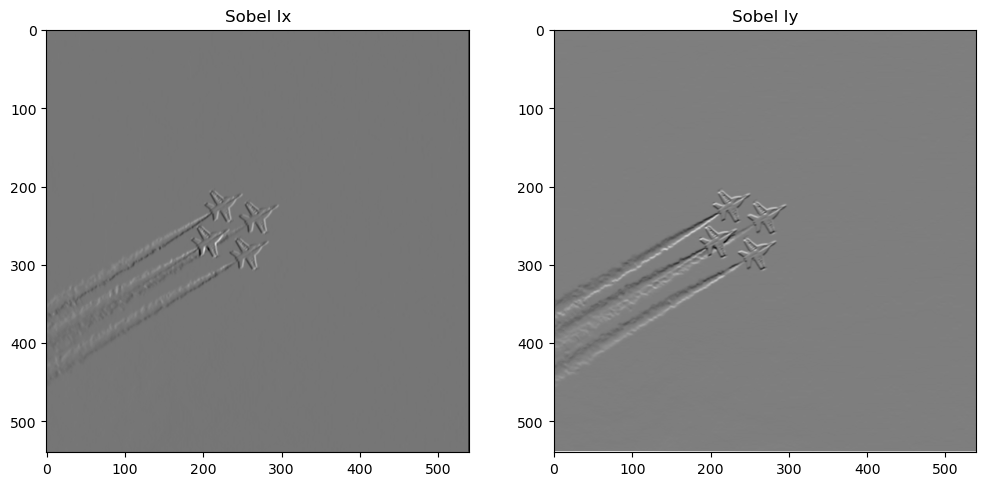
\includegraphics[width=0.6\linewidth]{images/gradients_sample.png}
    \caption{Example of what a Sobel kernel applied via convolution to an image in both x then y directions.}
    \label{fig:sobel_gradient}
\end{figure}

\begin{figure}[t]
    \centering
    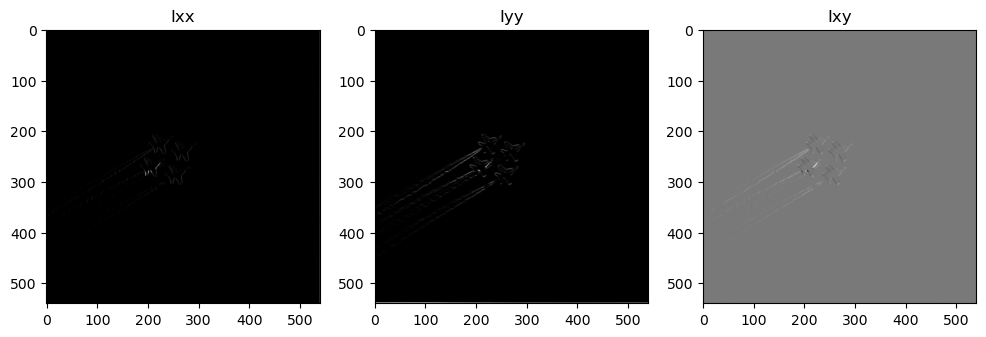
\includegraphics[width=0.95\linewidth]{images/pre_gaussian_low_pass_filters.png}
    \caption{Example of directional intensity changes from the Ixx, Iyy, and Ixy images.}
    \label{fig:pre_gaussian_lpf}
\end{figure}

\begin{figure}[t]
    \centering
    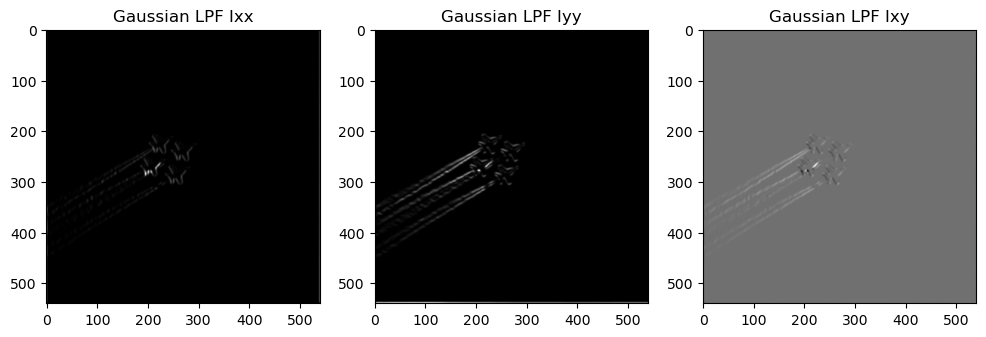
\includegraphics[width=0.95\linewidth]{images/gaussian_low_pass_filters.png}
    \caption{Example of Gaussian low-pass filters applied on the Ixx, Iyy, and Ixy images. The filters smooth the image in the respective directions, reducing high-frequency noise, ultimately aiding in the corner detection.}
    \label{fig:gaussian_lpf}
\end{figure}

\begin{figure}[h]
    \centering
    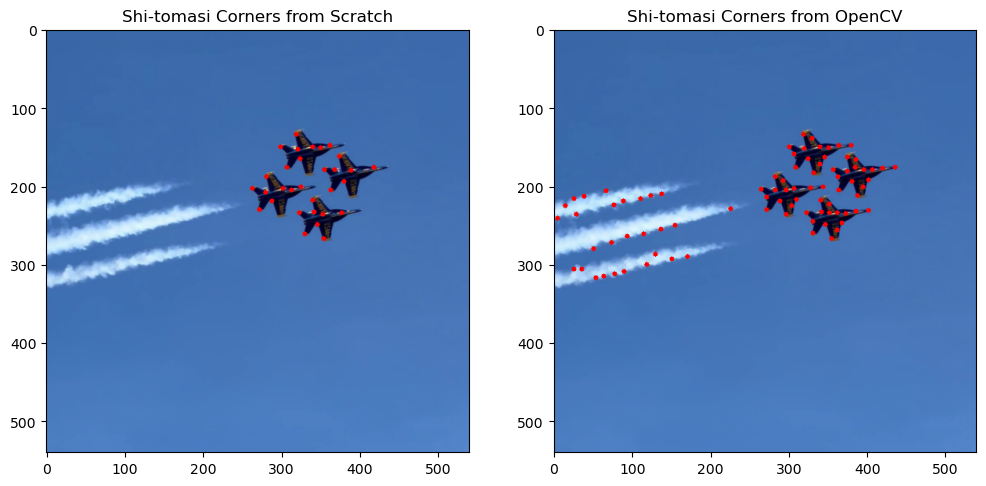
\includegraphics[width=0.95\linewidth]{images/shi_tomasi_corners.png}
    \caption{Detected corners using the Shi-Tomasi method. Left image is pure NumPy implementation, right image is OpenCV's goodFeaturesToTrack method. Red circles indicate detected corners overlaid on the input image (sensitivity is 0.04, max corners is 200).}
    \label{fig:shi_tomasi_results}
\end{figure}

\begin{figure}[h]
    \centering
    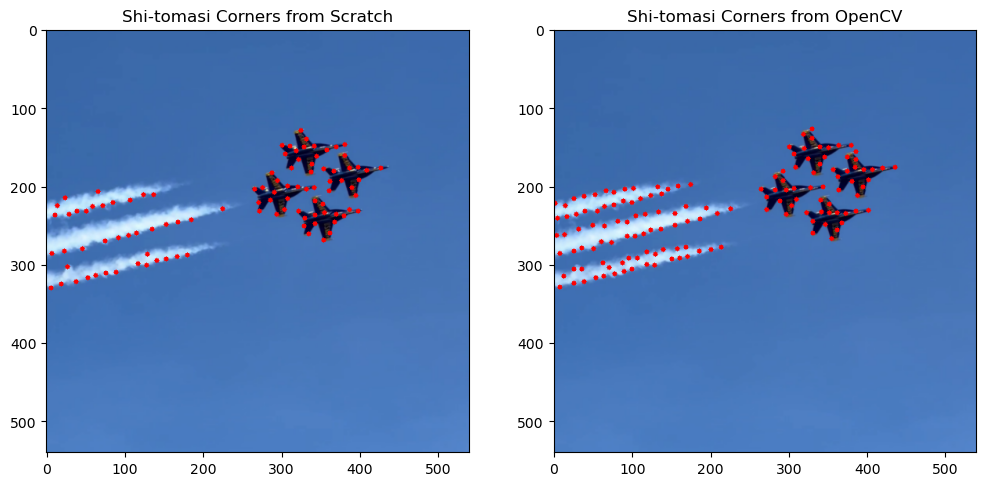
\includegraphics[width=0.95\linewidth]{images/shi_tomasi_corners_2.png}
    \caption{Detected corners using the Shi-Tomasi method. Left image is pure NumPy implementation, right image is OpenCV's goodFeaturesToTrack method. Red circles indicate detected corners overlaid on the input image (sensitivity is 0.004, max corners is 2000).}
    \label{fig:shi_tomasi_results2}
\end{figure}
\twocolumn

\begin{figure}[t]
    \centering
    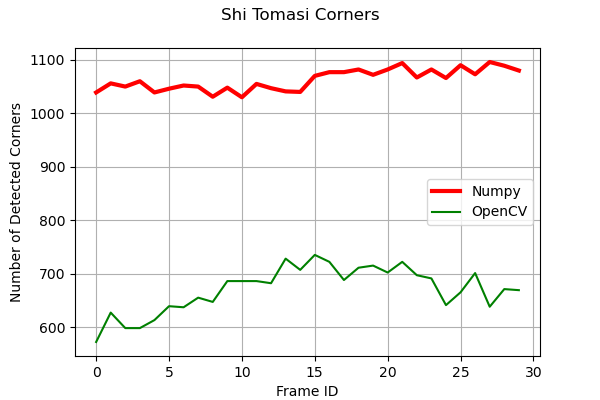
\includegraphics[width=\linewidth]{images/stc_corners.png}
    \caption{Number of corners detected between the algorithms.}
    \label{fig:stc-corners}
\end{figure}

\begin{figure}[t]
    \centering
    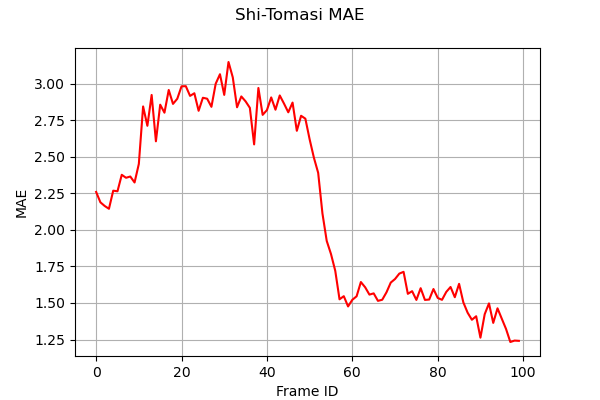
\includegraphics[width=\linewidth]{images/stc_mae.png}
    \caption{Mean absolute error between the images with corners plotted.}
    \label{fig:stc-mae}
\end{figure}

\begin{figure}[t]
    \centering
    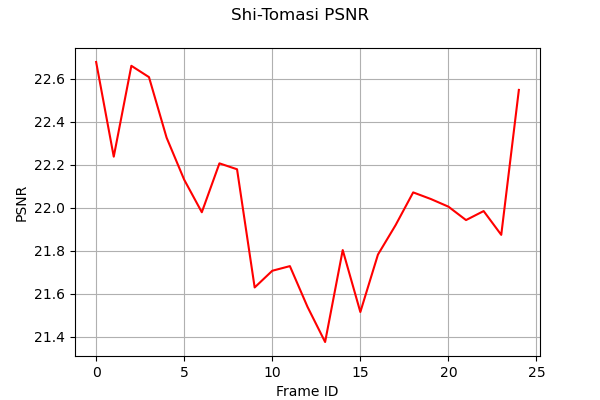
\includegraphics[width=\linewidth]{images/stc_psnr.png}
    \caption{Peak signal to noise ratio between images with corners plotted.}
    \label{fig:stc-psnr}
\end{figure}

\begin{figure}[t]
    \centering
    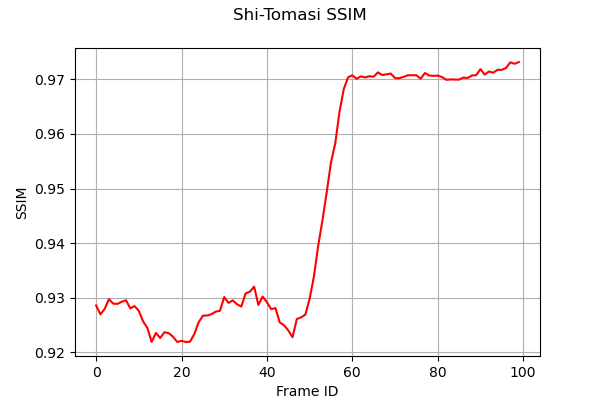
\includegraphics[width=\linewidth]{images/stc_ssim.png}
    \caption{Structural similarity index between images with corners plotted.}
    \label{fig:stc-ssim}
\end{figure}

\begin{figure}[t]
    \centering
    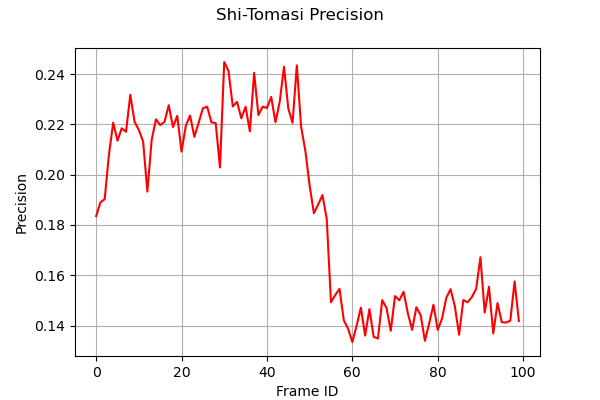
\includegraphics[width=\linewidth]{images/stc_precision.png}
    \caption{Precision calculations between all corners between algorithms (euclidean distance was used)}
    \label{fig:stc-prec}
\end{figure}

\begin{figure}[t]
    \centering
    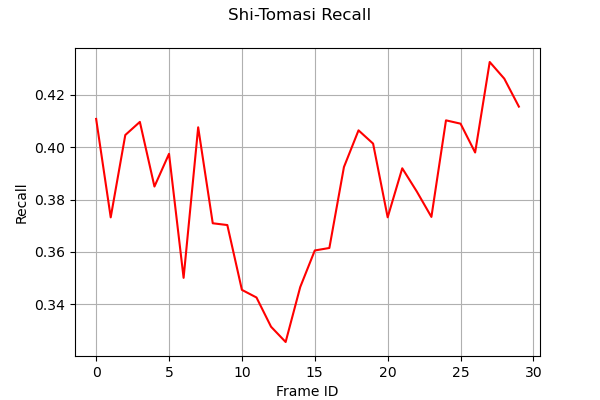
\includegraphics[width=\linewidth]{images/stc_recall.png}
    \caption{Recall calculations between all corners between algorithms (euclidean distance was used)}
    \label{fig:stc-rec}
\end{figure}

\onecolumn
\begin{lstlisting}[style=python, caption={Shi-Tomasi Corners Function}, label={lst:shi-tomasi}]
    def shi_tomasi_corners(img, max_corners=200, ksize=3, method='NumPy', sensitivity=0.04, sigma0=0, min_dist=10, debug=False, show_image=False, plots_dir=None):
    
        height, width = img.shape
        gray = np.float32(img)
            
        # Ix, Iy: Gradients in the x, y directions (horizontal/vertical changes).
        # Gradients highlight areas of rapid intensity change, which are corner candidates
        # Done by calculating the derivative of the intensity function
        # Compute image gradients (Ix, Iy) using Sobel filters
        Ix = gradient['NumPy'](gray.copy(), ksize, 0)
        Iy = gradient['NumPy'](gray.copy(), ksize, 1)
            
        # Compute elements of the covariance matrix
        # Ixx: Gradient squared in the x-direction (horizontal intensity change)
        # Iyy: Gradient squared in the y-direction (vertical intensity change)
        # Ixy: Product of gradients in both directions, showing thier interaction
        Ixx0 = Ix * Ix
        Iyy0 = Iy * Iy
        Ixy0 = Ix * Iy

        # Apply Gaussian filter to the matrix elements
        # The Gaussian blur is applied to smooth the covariance matrix elements. 
        # This step reduces noise and minor variations in the gradient images 
        # The kernel size for the Gaussian blur is determined by ksize, which is the same as that used for the Sobel operator. 
        # The smoothing ensures that the corner response is more robust by averaging local intensity variations.
        Ixx, sigma_xx = gaussian_low_pass['NumPy'](Ixx0, ksize, sigma0)
        Iyy, sigma_yy = gaussian_low_pass['NumPy'](Iyy0, ksize, sigma0)
        Ixy, sigma_xy = gaussian_low_pass['NumPy'](Ixy0, ksize, sigma0)
  
        # Compute the minimum eigenvalue (Shi-Tomasi score) for each pixel
        # det_M: This computes the determinant of the covariance matrix M
        # M = ([Ixx, Ixy], [Ixy, Iyy])
        # The determinant helps to identify the strength of the corners.
        # trace_M computes trace of the covariance matrix M (sum of its diagonal elements)
        # The final response is calculated using a combination of the determinant and trace.
        # The subtraction of <sensitivity>*trace_M^2 helps adjust the sensitivity of corner detection, ensuring that the corners detected are of high quality.
        det_M = Ixx * Iyy - (Ixy ** 2)
        trace_M = Ixx + Iyy
        response = det_M - (sensitivity * (trace_M ** 2))

        # Flatten the response matrix and get top N corners
        # Sort indices by highest values to determine the strongest corners
        flat_response = response.flatten()
        top_indices = np.argsort(flat_response)[-max_corners:]

        coords = np.array(np.unravel_index(top_indices, response.shape)).T
        filtered_coords = coordinate_density_filter(coords, min_dist, max_corners, height, width)

        coords_cv2 = cv2.goodFeaturesToTrack(image=img, maxCorners=max_corners, qualityLevel=sensitivity, minDistance=min_dist)
        coords_cv2 = np.array([(int(corner[0][1]), int(corner[0][0])) for corner in coords_cv2])
        filtered_coords_cv2 = coords_cv2
        
        return filtered_coords, filtered_coords_cv2
\end{lstlisting}

\begin{lstlisting}[style=python, caption={2-Dimensional Convolution Routine}, label={lst:convolution}]
    @jit(nopython=True)
    def apply_convolution(image, kernel):
        """Applies a 2D convolution to an image with the given kernel using Numba."""
        image_h, image_w = image.shape
        kernel_h, kernel_w = kernel.shape
        
        # Calculate padding size
        pad_h = kernel_h // 2
        pad_w = kernel_w // 2
        
        # Create a padded image
        padded_image_h = image_h + 2 * pad_h
        padded_image_w = image_w + 2 * pad_w
        padded_image = np.zeros((padded_image_h, padded_image_w), dtype=np.float32)
    
        # Fill the padded image with the original image
        for i in range(image_h):
            for j in range(image_w):
                padded_image[i + pad_h, j + pad_w] = image[i, j]
    
        # Prepare output image
        convolved_image = np.zeros_like(image, dtype=np.float32)
    
        # Perform convolution using nested loops
        for i in range(image_h):
            for j in range(image_w):
                # Extract interest region
                region = padded_image[i:i + kernel_h, j:j + kernel_w]
                # Apply the kernel to the region and sum the result
                convolved_image[i, j] = np.sum(region * kernel)
        
        return convolved_image
\end{lstlisting}

\begin{lstlisting}[style=python, caption={Sobel Kernel}, label={lst:sobel-kernel}]
    def create_sobel_operator(ksize, xy):

        if ksize % 2 == 0:
            raise ValueError("Kernel size must be odd.")
        
        # Create the base grid
        mid = ksize // 2
        x, y = np.meshgrid(np.arange(-mid, mid + 1), np.arange(-mid, mid + 1))
        
        # Sobel kernel calculations
        kx = x / (x**2 + y**2 + 1e-6)  # Small value added to avoid division by zero
        ky = y / (x**2 + y**2 + 1e-6)
        
        # Normalize kernels
        kx = kx / np.sum(np.abs(kx)) if np.sum(np.abs(kx)) != 0 else kx
        ky = ky / np.sum(np.abs(ky)) if np.sum(np.abs(ky)) != 0 else ky
        
        return kx if xy == 0 else ky
\end{lstlisting}

\newpage
\begin{lstlisting}[style=python, caption={Gaussian Kernel}, label={lst:gaussian-kernel}]
    def gaussian_kernel(size, sigma):
        """Generates a Gaussian kernel."""
                
        axis = np.linspace(-(size // 2), size // 2, size)
        kernel_1d = np.exp(-0.5 * (axis / sigma) ** 2)
        kernel_1d /= kernel_1d.sum()  # Normalize the kernel
        kernel_2d = np.outer(kernel_1d, kernel_1d)
        return kernel_2d
\end{lstlisting}

\begin{lstlisting}[style=python, caption={Corner Density Filter}, label={lst:corner_filter}]
    def coordinate_density_filter(coords, min_dist, max_corners, image_height, image_width, image_edge_threshold=5):
        # Enforce minimum distance constraint
        filtered_coords = []
        for coord in coords:
            if all(np.linalg.norm(coord - np.array(fc)) >= min_dist for fc in filtered_coords):
                filtered_coords.append(coord)
                if len(filtered_coords) >= max_corners:
                    break

        final_corners = []    
        for coord in filtered_coords:
            y, x = coord
            # Check if the point is not within the threshold of the edges
            if (x > image_edge_threshold and x < (image_width - image_edge_threshold) and
                y > image_edge_threshold and y < (image_height - image_edge_threshold)):
                final_corners.append(coord)

        return np.array(final_corners)
\end{lstlisting}
\twocolumn




%%%%%%%%%%%%%%%%%%%%%%%%%%%%%%%%%%%%%%%%%%%%%%%%%%%%%%%%%

\subsection{Lucas-Kanade Optical Flow}

The Lucas-Kanade Optical Flow algorith was used for tracking feature points in a video sequence. Specically a video snippet of Blue Angels Fighter Planes. The core of the implementation is based on the pyramidal Lucas-Kanade method, which is utilized both through OpenCV's built-in function (\texttt{cv2.calcOpticalFlowPyrLK}) and a custom NumPy-based implementation (\texttt{calcOpticalFlowPyrLK\_NumPy}).

\subsubsection{Key Parameters for Optical Flow}
The following parameters are used to configure the optical flow algorithm:
\begin{itemize}
    \item \textbf{Window Size:} Defines the size of the window used for local flow computation.
    \item \textbf{Pyramid Level:} Controls the resolution levels in the pyramid used for coarse-to-fine tracking.
    \item \textbf{Error Threshold:} The maximum allowable error for tracking. If the error exceeds this threshold, the feature is considered lost.
    \item \textbf{Reinitialization Threshold:} The minimum acceptable corners persisted from the previous frame, if there aren't enough corners to assess, then do not go through the optical flow calculations and simply detect more corners for the following frame
\end{itemize}
\bigskip

\subsubsection{Implementation Details}
% \subsubsection{Optical Flow Calculation}
The optical flow computation is performed across successive frames of a video. Given the previous and current frames, along with a set of feature points (typically corners detected in the first frame), the algorithm estimates the motion of these points. The Lucas-Kanade method computes the flow by solving the optical flow equation using image gradients. This method assumes that the flow is constant within a local neighborhood (region) of the pixel, which is a fundamental assumption of the method.

% \subsubsection{Pyramidal Representation}
To handle larger motions and improve performance, we use an image pyramid. The images are downscaled multiple times to create a series of progressively lower-resolution images. Flow is computed from the highest (smallest) resolution up to the original resolution. This approach helps in capturing large displacements efficiently.

% \subsubsection{Flow Calculation at Each Pyramid Level}
For each pyramid level, the flow is calculated by solving the system of equations derived from image gradients and temporal differences between frames. The gradients in both the x and y directions (\(I_x\) and \(I_y\)) are computed using Sobel operators. Temporal differences (\(I_t\)) are computed as the difference between the current and previous frames. These gradients are used to form the matrix \(\mathbf{A}\) and the vector \(\mathbf{b}\), which are then solved to estimate the motion vector for each point.

% \subsubsection{Multi-level Processing}
The optical flow is first computed at the smallest resolution (top of the pyramid), and the computed flow is propagated to larger resolutions by scaling the flow and adjusting the points accordingly. This multi-level approach allows for better handling of large motions.

% \subsubsection{Flow Calculation Using NumPy and OpenCV}
The function \texttt{calcOpticalFlowPyrLK\_NumPy} (see code list \ref{lst:calcOpticalFlowPyrLK}) is the custom NumPy-based implementation of the pyramidal Lucas-Kanade method, while \texttt{cv2.calcOpticalFlowPyrLK} uses OpenCV's optimized implementation. Both functions follow the same basic structure but differ in implementation. The NumPy version directly computes gradients and solves the flow equations, while OpenCV uses highly optimized C++ functions for these operations.

% \subsubsection{Point Tracking}
At each frame, the feature points are tracked from their position in the previous frame to their new position in the current frame. The \texttt{validate\_points} function (see code list \ref{lst:valpoints}) ensures that only valid points are kept (i.e., points that are successfully tracked). It checks the tracking status (\texttt{st}) and the error (\texttt{err}) against predefined thresholds to filter out unreliable tracks.

% \subsubsection{Reinitialization}
If the number of valid points falls below a threshold, or if the tracking quality degrades (as indicated by the error threshold), the system reinitializes the feature points using corner detection. This ensures that the tracker remains robust over time, even in challenging conditions.

\bigskip

\subsubsection{Visualization}
The tracked points are visually represented in a video where:
\begin{itemize}
    \item The top-left quadrant shows the feature points detected by the NumPy-based method.
    \item The top-right quadrant displays points detected by OpenCV's \texttt{cv2.goodFeaturesToTrack}.
    \item The bottom-left quadrant shows the points tracked by the NumPy-based Lucas-Kanade method
    \item The bottom-right quadrant shows the points tracked by OpenCV Lucas-Kanade method
\end{itemize}
The red points are simply the Shi-Tomasi corners (upper half of the images). The green points are considered good points tracked from one the previous frame to the current frame, and the red points are new corners added to the list of viable points for the optical flow calculations based on the reinitalization criteria. Figures \ref{fig:sample_1} through \ref{fig:sample_5} show a 5-frame sequence of corners being detected, and persisting over several frames, with many corners falling away and new corners being initizalized.
\bigskip

\subsubsection{Handling Edge Cases}
\begin{itemize}
    \item \textbf{Reinitialization:} If tracking fails due to the loss of too many points, the system reinitializes the points using the Shi-Tomasi corner detection method.
    \item \textbf{Error Thresholding:} An error threshold (\texttt{err\_thresh}) is used to filter out points with large tracking errors, ensuring that only reliable tracks are kept.
\end{itemize}
\bigskip

\subsubsection{Statistics Tracking}
The same metrics used in evaluating the Shi-Tomasi corner detection algorith were used for evaluating the Lucas-Kanade algorithms, only using images with the corners that were succesful in persiting through frames were recorded. Addtional metrics were created to record how often either algorithm attempted to validate points based on the given thresholds, as well as how often corners for the image were reinitalized. See Figures \ref{fig:lk-corners} through \ref{fig:lk-rec} for example output produced when processing a video of Blue Angels Fighters flying in their diamon formation.
\bigskip

\subsubsection{Performance Metrics}
During the processing of the video, the script keeps track of the number of feature points detected and tracked, as well as the number of reinitializations (when feature points are lost or tracking fails). These metrics are collected and saved for later analysis.
\bigskip

\onecolumn
\begin{figure}[t]
    \centering
    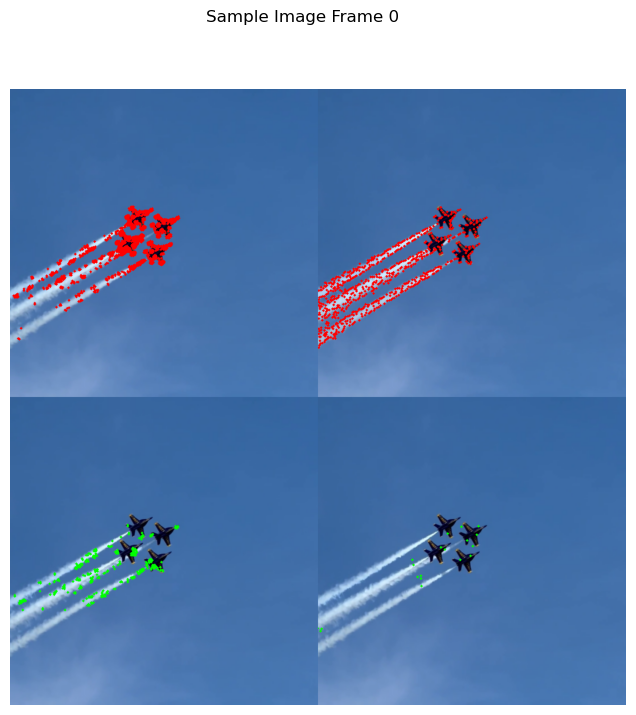
\includegraphics[width=0.8\linewidth]{images/sample_image_0.png}
    \caption{Upper half is detected corners using the Shi-Tomasi method. Bottom half is Lucas-Kanade good corners that persisted through the optical flow calculations. Left side is pure NumPy implementation, right side is OpenCV's calcOpticalFlowPyrLK method. Blue circles are simply all corners detected, green circles indicate good corners that have persisted between the previous frame to the current frame, and red circles are new corners initialized for the current frame if needed.}
    \label{fig:sample_1}
\end{figure}


\begin{figure}[h]
    \centering
    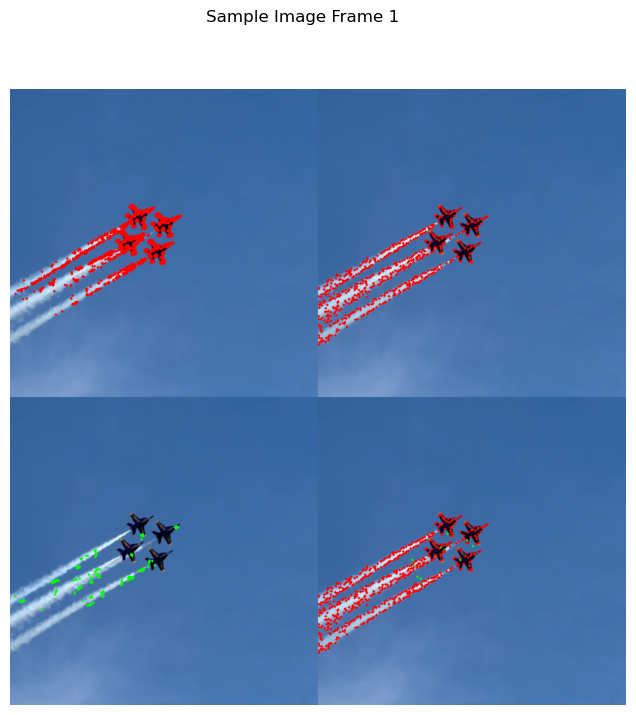
\includegraphics[width=0.8\linewidth]{images/sample_image_1.png}
    \caption{Upper half is detected corners using the Shi-Tomasi method. Bottom half is Lucas-Kanade good corners that persisted through the optical flow calculations. Left side is pure NumPy implementation, right side is OpenCV's calcOpticalFlowPyrLK method. Blue circles are simply all corners detected, green circles indicate good corners that have persisted between the previous frame to the current frame, and red circles are new corners initialized for the current frame if needed.}
    \label{fig:sample_2}
\end{figure}

\begin{figure}[h]
    \centering
    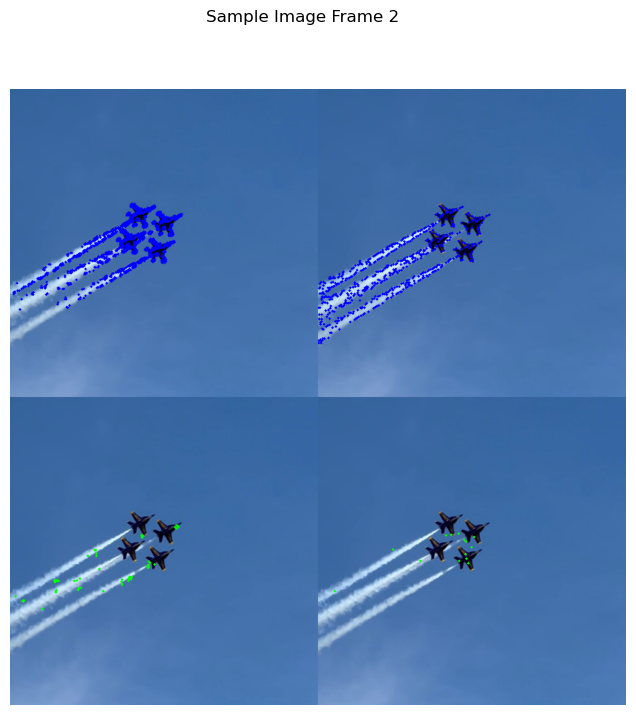
\includegraphics[width=0.8\linewidth]{images/sample_image_2.png}
    \caption{Upper half is detected corners using the Shi-Tomasi method. Bottom half is Lucas-Kanade good corners that persisted through the optical flow calculations. Left side is pure NumPy implementation, right side is OpenCV's calcOpticalFlowPyrLK method. Blue circles are simply all corners detected, green circles indicate good corners that have persisted between the previous frame to the current frame, and red circles are new corners initialized for the current frame if needed.}
    \label{fig:sample_3}
\end{figure}


\begin{figure}[h]
    \centering
    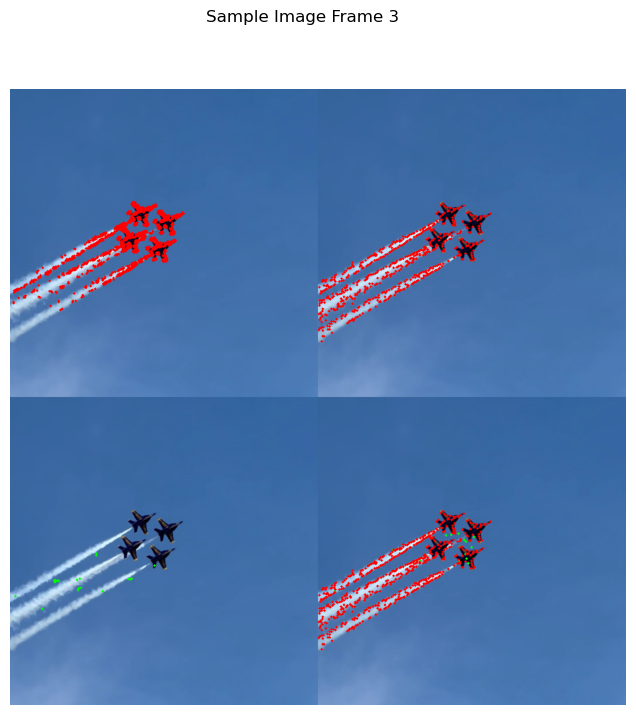
\includegraphics[width=0.8\linewidth]{images/sample_image_3.png}
    \caption{Upper half is detected corners using the Shi-Tomasi method. Bottom half is Lucas-Kanade good corners that persisted through the optical flow calculations. Left side is pure NumPy implementation, right side is OpenCV's calcOpticalFlowPyrLK method. Blue circles are simply all corners detected, green circles indicate good corners that have persisted between the previous frame to the current frame, and red circles are new corners initialized for the current frame if needed.}
    \label{fig:sample_4}
\end{figure}
\twocolumn

\onecolumn
\begin{figure}[h]
    \centering
    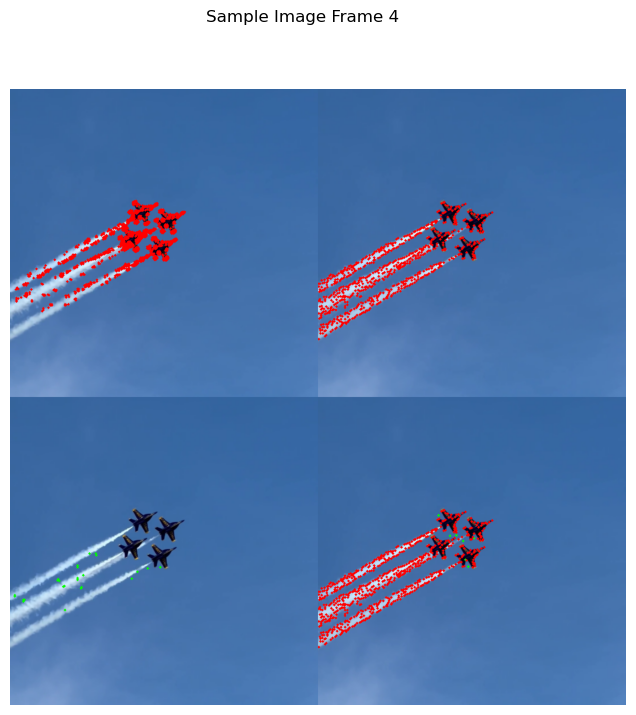
\includegraphics[width=0.8\linewidth]{images/sample_image_4.png}
    \caption{Upper half is detected corners using the Shi-Tomasi method. Bottom half is Lucas-Kanade good corners that persisted through the optical flow calculations. Left side is pure NumPy implementation, right side is OpenCV's calcOpticalFlowPyrLK method. Blue circles are simply all corners detected, green circles indicate good corners that have persisted between the previous frame to the current frame, and red circles are new corners initialized for the current frame if needed.}
    \label{fig:sample_5}
\end{figure}
\twocolumn

\begin{figure}[t]
    \centering
    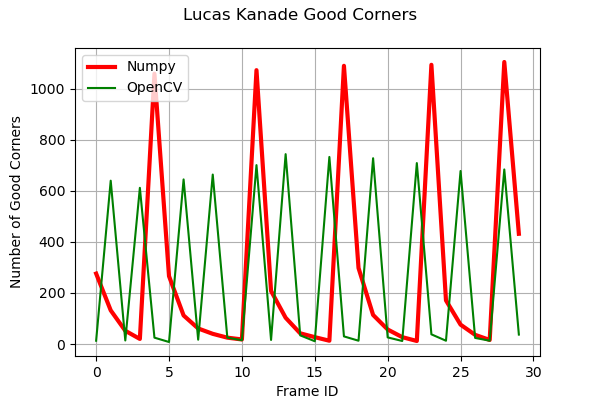
\includegraphics[width=0.9\linewidth]{images/lk_good_corners.png}
    \caption{Number of good corners remaining after optical flow calculations between the algorithms.}
    \label{fig:lk-corners}
\end{figure}

\begin{figure}[t]
    \centering
    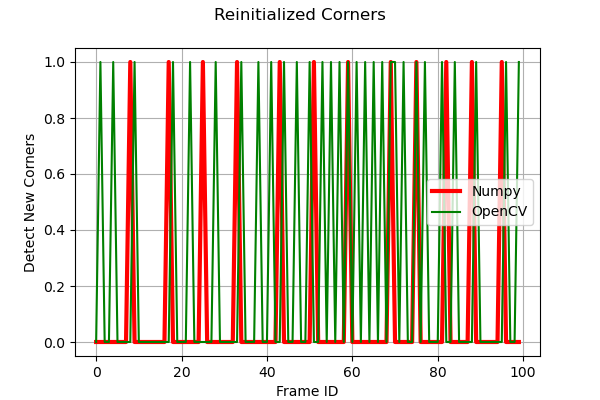
\includegraphics[width=0.9\linewidth]{images/reinits.png}
    \caption{Times when not enough corners persisted, and the algorithm had to reinitialize points.}
    \label{fig:lk-reinits}
\end{figure}

\begin{figure}[t]
    \centering
    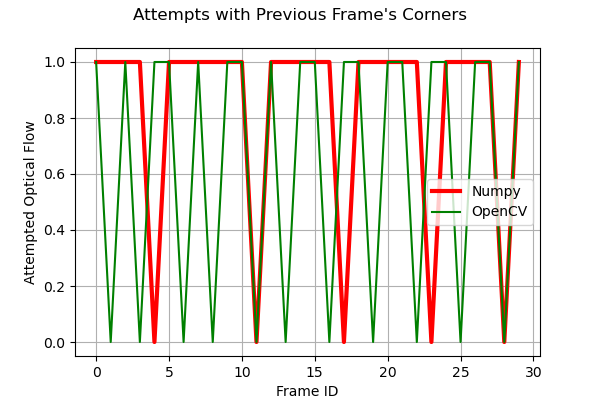
\includegraphics[width=0.9\linewidth]{images/attempts.png}
    \caption{Times when attempts to go through the optical flow calculations were taken.}
    \label{fig:lk-attempts}
\end{figure}

\begin{figure}[t]
    \centering
    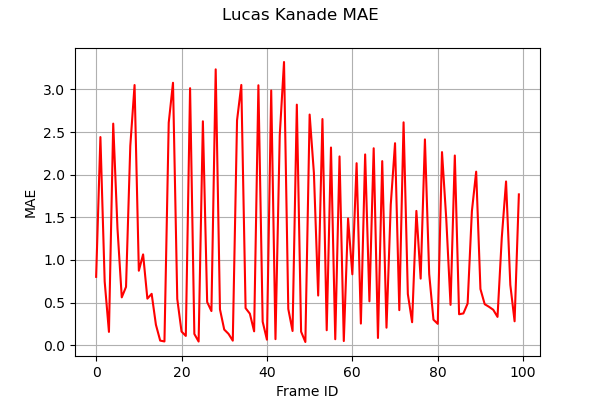
\includegraphics[width=0.9\linewidth]{images/lk_mae.png}
    \caption{Mean absolute error between the images with corners plotted.}
    \label{fig:lk-mae}
\end{figure}

\begin{figure}[t]
    \centering
    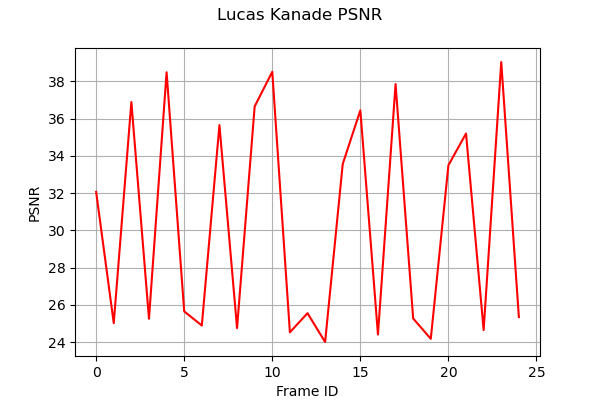
\includegraphics[width=0.9\linewidth]{images/lk_psnr.png}
    \caption{Peak signal to noise ratio between images with corners plotted.}
    \label{fig:lk-psnr}
\end{figure}

\begin{figure}[t]
    \centering
    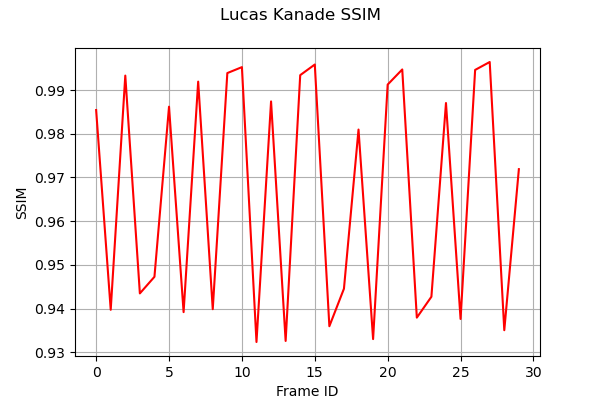
\includegraphics[width=0.9\linewidth]{images/lk_ssim.png}
    \caption{Structural similarity index between images with corners plotted.}
    \label{fig:lk-ssim}
\end{figure}

\onecolumn

\begin{figure}[t]
    \centering
    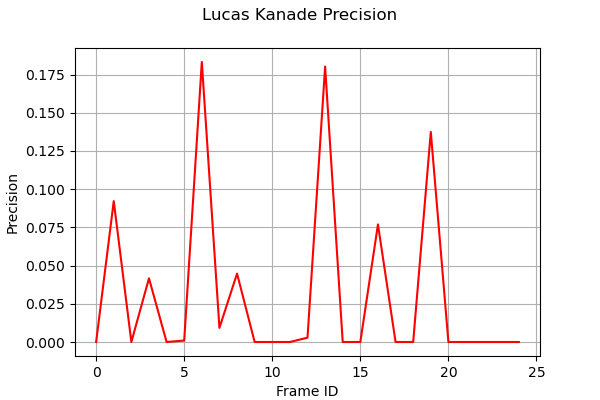
\includegraphics[width=0.45\linewidth]{images/lk_precision.png}
    \caption{Precision calculations between all good corners between algorithms (euclidean distance was used)}
    \label{fig:lk-prec}
\end{figure}

\begin{figure}[t]
    \centering
    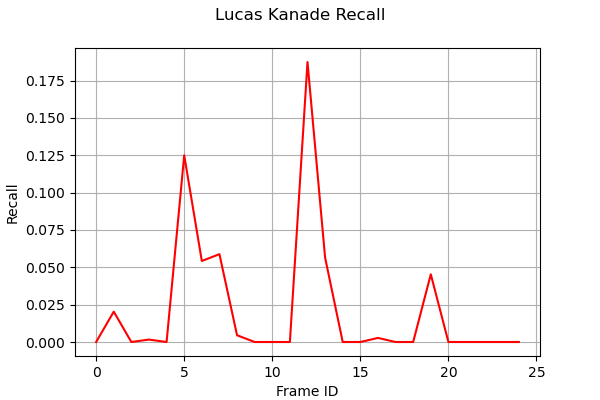
\includegraphics[width=0.45\linewidth]{images/lk_recall.png}
    \caption{Recall calculations between all good corners between algorithms (euclidean distance was used)}
    \label{fig:lk-rec}
\end{figure}


\onecolumn
\begin{lstlisting}[style=python, caption={\texttt{calcOpticalFlowPyrLK\_NumPy}}, label={lst:calcOpticalFlowPyrLK}]
    def calcOpticalFlowPyrLK_NumPy(prev_img, curr_img, points_prev, lk_params=None, ksize=3, method='NumPy'):

    winSize, maxLevel, criteria = lk_params.values()
    __, max_iter, epsilon = criteria
    
    # Initialize variables for flow tracking
    points_curr = np.copy(points_prev)  # Initial flow starts as the initial points
    st = np.ones(len(points_prev), dtype=np.uint8)  # Status array
    err = np.zeros(len(points_prev), dtype=np.float32)  # Error array

    # Build image pyramids for previous and current frames
    pyramid_prev = [prev_img]
    pyramid_curr = [curr_img]
    for i in range(1, maxLevel + 1):
        pyramid_prev.append(cv2.pyrDown(pyramid_prev[i - 1]))
        pyramid_curr.append(cv2.pyrDown(pyramid_curr[i - 1]))

    # Start processing from the top of the pyramid (smallest scale)
    scale_factor = 2 ** maxLevel
    for level in range(maxLevel, -1, -1):
        # Scale down point coordinates for current pyramid level
        points_prev_scaled = points_prev / scale_factor
        points_curr_scaled = points_curr / scale_factor
        half_w, half_h = winSize[0] // 2, winSize[1] // 2

        for i, point in enumerate(points_prev_scaled):
            # Extract patches around the points
            x, y = int(point[0][0]), int(point[0][1])
            try:
                prev_patch = pyramid_prev[level][y - half_h:y + half_h + 1, x - half_w:x + half_w + 1]
                curr_patch = pyramid_curr[level][y - half_h:y + half_h + 1, x - half_w:x + half_w + 1]
            except IndexError as e:
                st[i] = 0
                continue

            # Proceed if patches match the specified window size
            if prev_patch.shape == winSize and curr_patch.shape == winSize:
                # Compute gradients and temporal difference
                Ix = gradient[method](prev_patch, ksize=ksize, xy=0)
                Iy = gradient[method](prev_patch, ksize=ksize, xy=1)
                It = curr_patch.astype(np.float32) - prev_patch.astype(np.float32)

                # Calculate terms for solving the optical flow equation
                Ixx = Ix ** 2
                Iyy = Iy ** 2
                Ixy = Ix * Iy
                Ixt = Ix * It
                Iyt = Iy * It
                A = np.array([[Ixx.sum(), Ixy.sum()], [Ixy.sum(), Iyy.sum()]])
                b = -np.array([Ixt.sum(), Iyt.sum()])

                # Iteratively solve for optical flow
                flow = np.zeros(2)
                for _ in range(max_iter):
                    if np.linalg.det(A) > 1e-5:
                        new_flow = np.linalg.solve(A, b)
                        if np.linalg.norm(new_flow - flow) < epsilon:
                            break
                        flow = new_flow
                    else:
                        st[i] = 0  # Mark tracking as failed
                        flow = np.zeros(2)
                        break

                # Update scaled points with the calculated flow
                points_curr_scaled[i][0][0] += flow[0]
                points_curr_scaled[i][0][1] += flow[1]
                err[i] = np.abs(It).mean()

        # Rescale points back to the original resolution
        points_curr += (points_curr_scaled * scale_factor - points_curr) / scale_factor
        scale_factor //= 2

    # Convert results to the expected formats
    points_curr = np.array(points_curr, dtype=np.float32)
    st = st.reshape(-1, 1)
    err = err.reshape(-1, 1)
    return points_curr, st, err
\end{lstlisting}

\begin{lstlisting}[style=python, caption={\texttt{validate\_points}}, label={lst:valpoints}]
    def validate_points(points_prev_0, points_curr, st, err, points_prev, err_thresh, image):
        
        reinit = 0
        if points_curr is not None and st is not None:                
            valid_mask = st.flatten() == 1
            
            # Filter points based on the valid mask
            good_new = points_curr[valid_mask]
            good_old = points_prev_0[valid_mask]
            err_valid = err[valid_mask]

            # Further filter based on error threshold using the same mask
            err_mask = err_valid.flatten() < err_thresh

            # Final filtering
            good_new = good_new[err_mask]
            good_new = good_new.reshape(len(good_new), 2)
            good_old = good_old[err_mask]
            good_old = good_old.reshape(len(good_old), 2)
            
            ## Draw the tracks on the color frame
            for i, (new, old) in enumerate(zip(good_new, good_old)):
                y1, x1 = map(int, new.ravel())
                y2, x2 = map(int, old.ravel())
                image = draw_corner_markers(image, [(y1, x1)], vid.green)  # Green markers

            points_prev_0 = vid.reshape_points(good_new)
            
            if type(points_prev_0) == type(None):
                image = draw_corner_markers(image, np.squeeze(points_prev), vid.red)
                points_prev_0 = points_prev
                reinit = 1
        else:
            ## Reinitialize points if tracking fails
            image = draw_corner_markers(image, np.squeeze(points_prev_0), vid.green)
            image = draw_corner_markers(image, np.squeeze(points_prev), vid.red)
            points_prev_0 = np.append(points_prev_0, points_prev, axis=0)
            reinit = 1

        return image, points_prev_0, reinit
\end{lstlisting}
\twocolumn

\section{Experimental Results}
In order to assess the performance of the NumPy and OpenCV KLT algorithms as a whole, a Monte Carlo tesing architecture was written. The same input video was used for all tests. The test setup begins by seeding a random number generator to ensure reproducibility of results. The video used for the anlysis was a Blue Angels Diamond Formation video (source \cite{Pexels:FighterJets}).

\subsection{Monte Carlo Parameters}

Monte Carlo simulation involves running 100 seeds (runs), each with randomized parameter values sampled from predefined distributions. The following parameters are used:
\begin{itemize}
    \item \textbf{max\_corners}: Uniform random integers between 2500 and 5000.
    \item \textbf{kernel\_size}: Random selection of odd integers from $\{3, 5, 7\}$.
    \item \textbf{gaussian\_sigma}: Uniform random floats in the range $[0, 2]$, rounded to six decimals.
    \item \textbf{corner\_sensitivity}: Uniform random floats in the range $[0.0005, 0.005]$, rounded to six decimals.
    \item \textbf{minimum\_distance}: Uniform random integers between 1 and 5.
    \item \textbf{reinit\_threshold}: Uniform random integers between 10 and 25.
    \item \textbf{window\_size}: Random selection of odd integers from $\{3, 5, 7\}$.
    \item \textbf{error\_threshold}: Uniform random floats in the range $[0.7, 0.9]$, rounded to six decimals.
    \item \textbf{pyrdown\_level}: Random selection of integers from $\{2, 3, 4\}$.
\end{itemize}

A histogram was generated to visualize the distributions of these parameters, to ensure they match the desired inputs, see Figure \ref{fig:mc_hist}.

\begin{figure}[t]
    \centering
    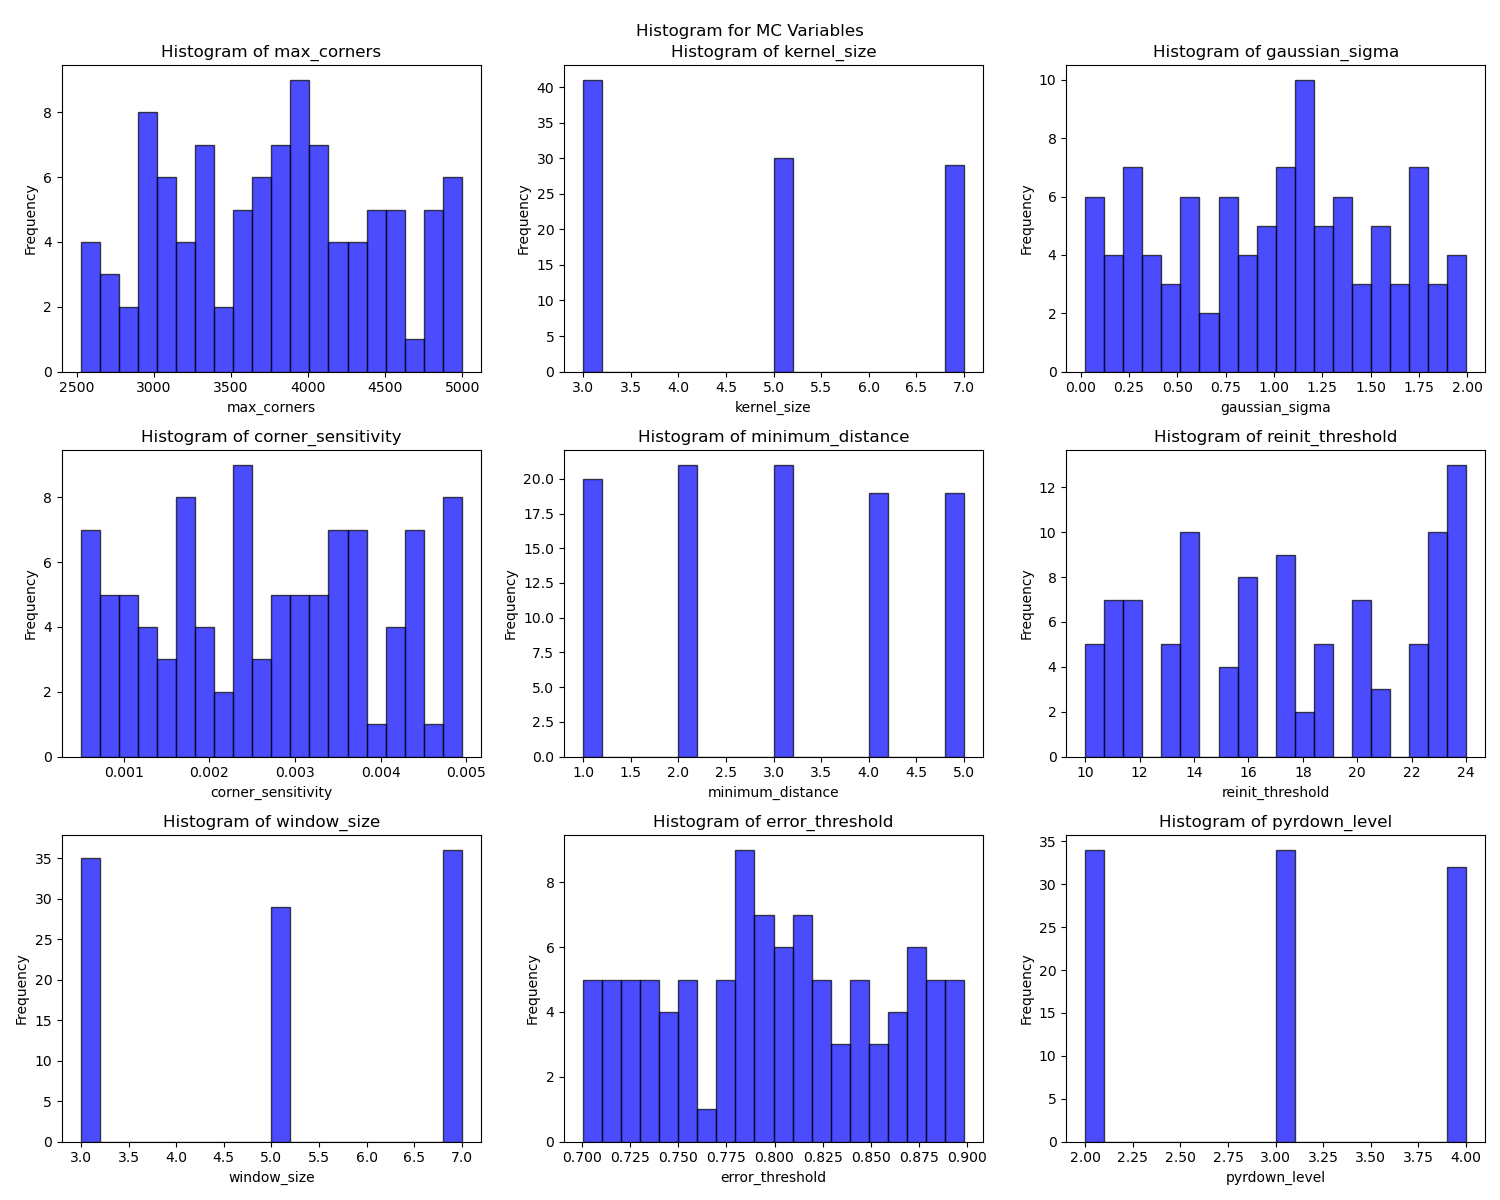
\includegraphics[width=\linewidth]{mc_images/mc_histogram.png}
    \caption{Histogram of all the Monte Carlo variables used and their distributions.}
    \label{fig:mc_hist}
\end{figure}

\subsection{Processing and Analysis}

For each run, parameters are passed to the Lucas-Kanade algorithm via the \texttt{lucas\_kanade\_optical\_flow} function (found in the Appendix as code list \ref{lst:lk}). Key features include:
\begin{itemize}
    \item Corner detection using Shi-Tomasi with the monte carlo randomized parameters.
    \item Optical flow computation with Lucas-Kanade using varied window sizes and pyramid levels.
\end{itemize}

The following metrics are captured and plotted against the other Monte Carlo seed runs:
\begin{itemize}
    \item Number of frames processed.
    \item Reinitializations for corner detection.
    \item Attempts to use previously detected corners for optical flow.
    \item Quality metrics including Mean Absolute Error (MAE), Peak Signal-to-Noise Ratio (PSNR), Structural Similarity Index Measure (SSIM), Precision, and Recall.
\end{itemize}

The results for these 50 Monte Carlo seeds are shown in Figures \ref{fig:mc_stc_mae} through \ref{fig:mc_lk_rec}

\begin{figure}[h!]
    \centering
    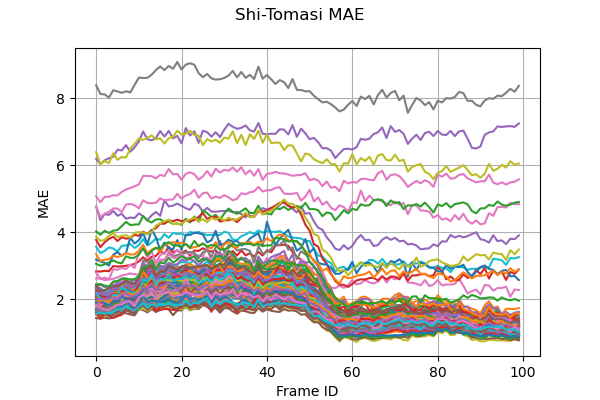
\includegraphics[width=\linewidth]{mc_images/mc_stc_mae.png}
    \caption{Mean absolute error between images with corners for all seeds.}
    \label{fig:mc_stc_mae}
\end{figure}

\begin{figure}[h!]
    \centering
    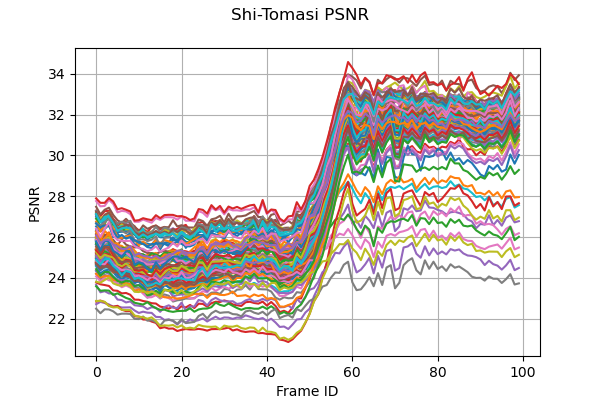
\includegraphics[width=\linewidth]{mc_images/mc_stc_psnr.png}
    \caption{Peak signal to noise ratio between images with corners for all seeds.}
    \label{fig:mc_stc_psnr}
\end{figure}

\begin{figure}[h!]
    \centering
    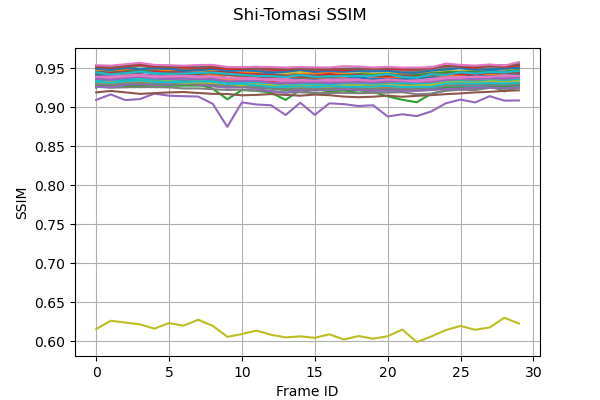
\includegraphics[width=\linewidth]{mc_images/mc_stc_ssim.png}
    \caption{Structural similarity index between images with corners for all seeds.}
    \label{fig:mc_stc_ssim}
\end{figure}

\begin{figure}[h!]
    \centering
    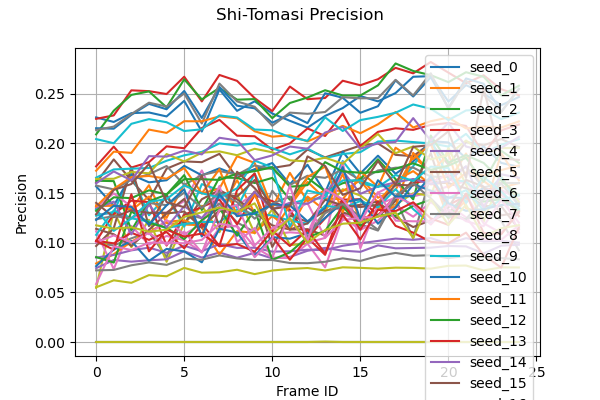
\includegraphics[width=\linewidth]{mc_images/mc_stc_precision.png}
    \caption{Precision calculations between all corners between algorithms (euclidean distance was used) for all seeds.}
    \label{fig:mc_stc_prec}
\end{figure}

\begin{figure}[h!]
    \centering
    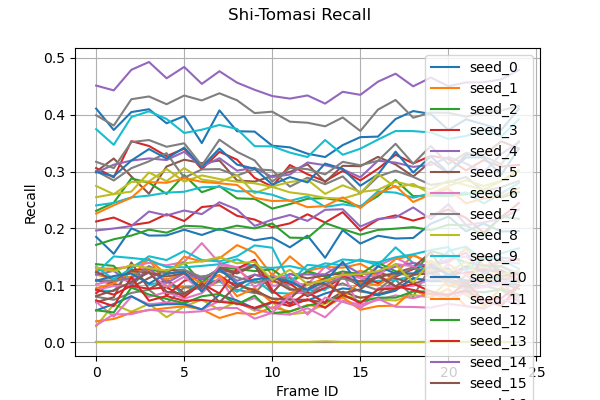
\includegraphics[width=\linewidth]{mc_images/mc_stc_recall.png}
    \caption{Recall calculations between all corners between algorithms (euclidean distance was used) for all seeds.}
    \label{fig:mc_stc_rec}
\end{figure}

\begin{figure}[h!]
    \centering
    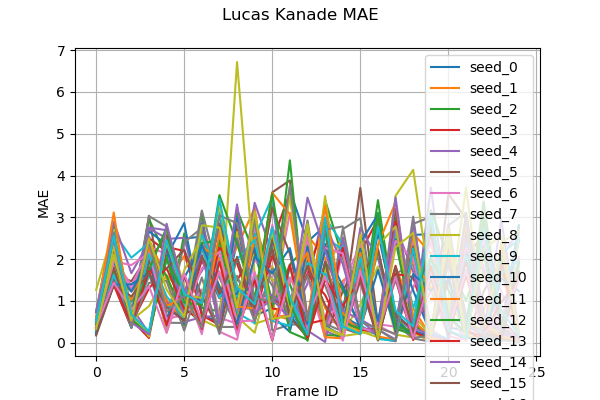
\includegraphics[width=\linewidth]{mc_images/mc_lk_mae.png}
    \caption{Mean absolute error between images with corners for all seeds.}
    \label{fig:mc_lk_mae}
\end{figure}

\begin{figure}[h!]
    \centering
    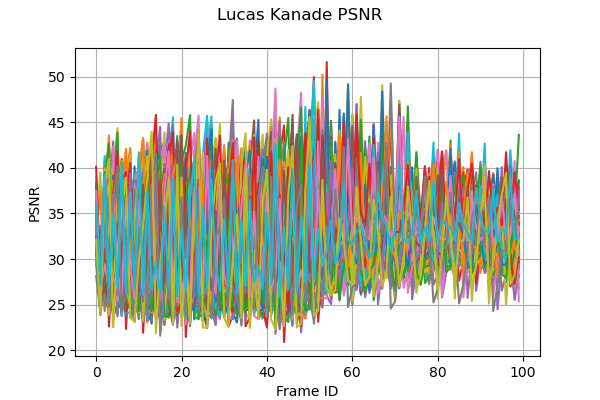
\includegraphics[width=\linewidth]{mc_images/mc_lk_psnr.png}
    \caption{Peak signal to noise ratio between images with corners for all seeds.}
    \label{fig:mc_lk_psnr}
\end{figure}

\begin{figure}[h!]
    \centering
    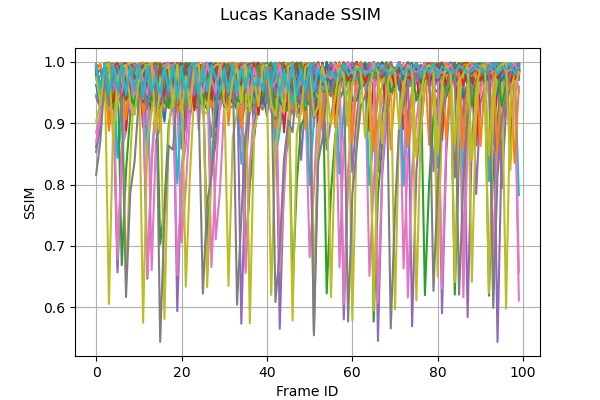
\includegraphics[width=\linewidth]{mc_images/mc_lk_ssim.png}
    \caption{Structural similarity index between images with corners for all seeds.}
    \label{fig:mc_lk_ssim}
\end{figure}

\begin{figure}[h!]
    \centering
    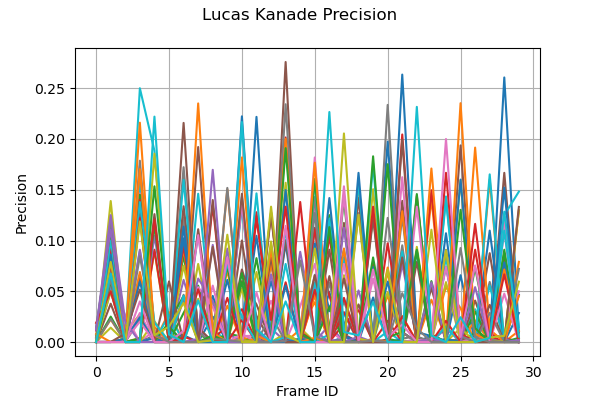
\includegraphics[width=\linewidth]{mc_images/mc_lk_precision.png}
    \caption{Precision calculations between all good corners between algorithms (euclidean distance was used) for all seeds.}
    \label{fig:mc_lk_prec}
\end{figure}

\begin{figure}[h!]
    \centering
    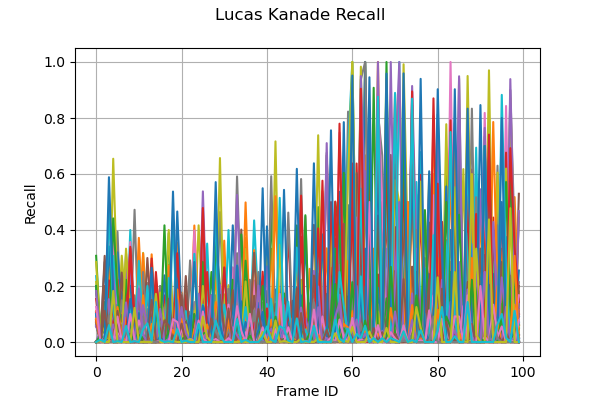
\includegraphics[width=\linewidth]{mc_images/mc_lk_recall.png}
    \caption{Recall calculations between all good corners between algorithms (euclidean distance was used) for all seeds.}
    \label{fig:mc_lk_rec}
\end{figure}

\section{Discussion}
Through basic evaluation of the algorithms developed in NumPy in this project and the optimized OpenCV implementation, they have good performance matching overall for 50 Monte Carlo seeds. Both are detecting good corners with good precision and recall scores between the corners detected and corners persisting through the optical flow calculations. Overall, the NumPy KLT algorithm works as intended and with more studies focused on optimization, the results would prove to more closely match the OpenCV algorithms.

The key players determined in the analysis of the Shi-Tomasi corner detection algorithm are three-fold, being the number of allowable corners detected, and the sensitivty threshold used with the eigavalue calculations, and the gaussin sigma value used in the low pass filter. Mixing in the other variables will shift the results around, but not to the same degree as these two variables. A much more in depth study should be conducted to determine at what combinations of these variables caused the algorithm to not perform.

A Gaussian low-pass filter alters the frequency content of a signal by attenuating high-frequency components. The parameter \(\sigma\) directly impacts the filter's behavior in both the spatial and frequency domains.



Big factors playing a role on the success of detected corners persisting over multiple frames of the video are the error threshold, reinit threshold, and overall the type of video. For objects that are moving extremely fast, this algorithm is not suited well for that.

Overall this project has forced a great deal of learning about how different image processing techniques influence how data can be extracted. The simple low pass filter used for the Shi-Tomasi corners plays a huge role in sharpenig the edges of the objects in the image, ultimately leading to better eigevalue scores where the corners should be predicted.

\bigskip

\section{Conclusions and Future Work}
This project demonstrates the practical implementation of the KLT feature tracker, highlighting its effectiveness and limitations. Future work could explore integrating advanced outlier rejection methods as well as further statistical methods for analyizing the points detected and better propogating them through time (and space). Ideas from the book Design and Analysis of Modern Tracking Systems by Robert Popoli and Samuel S. Blackamn would be a great start.

Additional work would be on the analysis side of this project, doing a correlation analysis to identify parameter sensitivity, and determine the best combinations of parameters that help the two algorithms (Shi-Tomasi and Lucas-Kanade) truly work in harmony as the Kanade-Lucas-Tomasi algorithm is designed to do.


\begin{thebibliography}{1}

    \bibitem{ShiTomasi}
    J. Shi and C. Tomasi, "Good features to track" in *Proc. IEEE Conf. Computer Vision and Pattern Recognition*, 1994, pp. 593-600.
    
    \bibitem{LucasKanade}
    B. D. Lucas and T. Kanade, "An iterative image registration technique with an application to stereo vision," in *Proc. Intl. Joint Conf. on Artificial Intelligence*, 1981, pp. 674-679.
    
    \bibitem{OpenCV}
    G. Bradski and A. Kaehler, *Learning OpenCV: Computer Vision with the OpenCV Library*. O'Reilly Media, 2008.
    
    \bibitem{Tan:Digital_Signal_Processing} 
    L. Tan, \textit{Digital Signal Processing}, INAOEP, 2013. [Online]. Available: \url{https://www-elec.inaoep.mx/~jmram/Digital_Signal_Processing__LI_TAN.pdf}.
    
    \bibitem{Wikipedia:KLT} 
    "Kanade-Lucas-Tomasi feature tracker," \textit{Wikipedia}, 2023. [Online]. Available: \url{https://en.wikipedia.org/wiki/Kanade%E2%80%93Lucas%E2%80%93Tomasi_feature_tracker}.
    
    \bibitem{Oppenheim:Schafer} 
    A. V. Oppenheim and R. W. Schafer, \textit{Discrete-Time Signal Processing}, 3rd ed., Pearson, 2010.
    
    \bibitem{KLT:Original}
    C. Kanade, T. Lucas, and B. Tomas, "An improved optical flow algorithm" in \textit{Proceedings of the IEEE Conference on Computer Vision and Pattern Recognition}, 1987, pp. 12-21. [Online]. Available: \url{https://ieeexplore.ieee.org/stamp/stamp.jsp?tp=&arnumber=6716443}.
    
    \bibitem{Pexels:FighterJets}
    Pexels, "Fighter Jets in Blue Sky," [Online]. Available: \url{https://www.pexels.com/video/fighter-jets-in-blue-sky-12954782/}. Accessed: Dec. 7, 2024.

\end{thebibliography}


\newpage

\onecolumn
\appendix
\subsection{Time Log for Project Development}

\begin{itemize}
    \item \textbf{2024-10-05}: Played with cv2 library in python importing videos and converting to grayscale (2 hours)
    \item \textbf{2024-10-06}: Played with cv2 library more (1 hour)
    \item \textbf{2024-10-07}: Created a sobel operator from scratch to use for calculating gradients of the images (2.5 hours)
    \item \textbf{2024-10-08}: Played with cv2 library using built-in commands for corner detection on an image (4 hours)
    \item \textbf{2024-10-10}: Developed debugging portions, committed testing scripts to git (2 hours)
    \item \textbf{2024-10-21}: Developed convolution routine from scratch (3 hours)
    \item \textbf{2024-10-28}: Hooked up convolution routine with kernels and made it work with sobel operators and other filters (very generic) (4.5 hours)
    \item \textbf{2024-11-01}: Corner detection algorithm development (Shi-Tomasi corners) (12.5 hours)
    \begin{itemize}
        \item Developed Shi-Tomasi code for both numpy and cv2 implementations, including error checking code
        \item Added plotting to show difference between home-grown solution for corner detection vs OpenCV module
        \item Added k-means clustering method for grouping detected points for the purpose of drawing bounding boxes
        \item Added several basic image transformations including high/low pass filters, and histogram equalization
        \item Added code for drawing uniform plots
        \item Added debugging code for evaluating metrics between image operations during intermediate steps
    \end{itemize}
    \item \textbf{2024-11-02}: Polished the Shi-Tomasi method a little more, and took a stab at implementing the optical flow portion of the Lucas-Kanade algorithm (4.5 hours)
    \item \textbf{2024-11-04}: Developed further the Lucas-Kanade method (OpenCV portion) and generated a video utilities file to use for generic function calls. Ready to convert to implementing the Lucas-Kanade algorithm from scratch now that the wrapper for the results is flushed out. (4.75 hours)
    \item \textbf{2024-11-05}: Developed algorithm for calcOpticalFlowPyrLK method, using the same inputs as the cv2 method. Now I have a fully functional custom KLT algorithm and a cv2 implementation. Next steps are making the custom method run solely on numpy operators, as well as quantifying performance between it, and adding comments throughout to discuss the math behind each operation. (7 hours)
    \item \textbf{2024-11-10}: Working on adding numpy versioning to the Lucas-Kanade algorithm (now fully numpy convolutions can be used) as well as added a frame skipping routine and a recursive pyrdown image operation to make the images smaller and therefore faster to calculate on (5.5 hours)
    \item \textbf{2024-11-15}: Revisited code for corner detections, made it work by testing both baseline and custom methods for corners (3 hours)
    \item \textbf{2024-11-18}: Worked on code cleanup (2 hours)
    \item \textbf{2024-11-21}: Developed video utilities to better work with the code base, more generic now (3 hours)
    \item \textbf{2024-11-22}: Worked on plotting functions to come up with methods to figure out how to best plot the corners detected (nearest neighbor, k-means clustering, Euclidean distance grouping) (4 hours)
    \item \textbf{2024-11-25}: Worked on testing metric ideas (2 hours)
    \item \textbf{2024-12-02}: Updated code for all image operations to be more generic, only working with a single image at a time (2.5 hours)
    \begin{itemize}
        \item Started final report (1.5 hours)
        \item Developed testing metrics for cv2 implementation versus numpy implementation
        \item Split focus between corners, persisting corners, and corner location (number of corners over all)
        \item Developed testing metric plots (2 hours)
        \item Reworked convolution algorithm (1.5 hour)
    \end{itemize}
    \item \textbf{2024-12-03}: Developed method for output images to be in quadrants (3 hours)
    \item \textbf{2024-12-03}: Developed MC analysis script for evaluating performance overall (3 hours)
    \item \textbf{2024-12-03}: Developed PSNR, MAE, SSIM, precision, and recall methods for images to be evaluated against each other (3.5 hours)
    \item \textbf{2024-12-04}: Connected MC script to Lucas-Kanade script in order to generate data and plots that show the results from each seed compared to the others (3.5 hours)
    \item \textbf{2024-12-04}: Also updated time-keeping sheet
    \item \textbf{2024-12-06}: Wrote report, adding images, plots, theory, code snippets, and explanations about code and my implementations of it (9.5 hours)
    \item \textbf{2024-12-07}: Finalized report with update images, and added more theory related to the low pass filters used in the corner detection algorithm (6.5 hours)
\end{itemize}
\bigskip

\subsection{Full Python Code Implementation}
For this project, all of the code has been implemented from scratch, including the video and image reading, writing, converting, processing, etc., various plotting scripts, image transormations, Monte-Carlo analysis, Shi-Tomasi corners, Lucas-Kanade optical flow, etc.

\begin{itemize}
    \item \texttt{monte\_carlo\_analysis.py} (code list \ref{lst:mc})
    \item \texttt{shi\_tomasi\_corners.py} (code list \ref{lst:stc})
    \item \texttt{image\_utils.py} (code list \ref{lst:iutils})
    \item \texttt{lucas\_kanade.py} (code list \ref{lst:lk})
    \item \texttt{video\_utils.py} (code list \ref{lst:vutils})
    \item \texttt{plot\_utils.py} (code list \ref{lst:putils})
    \item \texttt{utils.py} (code list \ref{lst:utils})
\end{itemize}

\begin{lstlisting}[style=python, caption={\texttt{monte\_carlo\_analysis.py}}, label={lst:mc}]
    import NumPy as np
    import lucas_kanade as lk
    import cv2
    from plot_utils import create_histogram, plot_mc_stats, plot_mc_error, plot_error
    import os
    from copy import copy
    from tqdm import tqdm
    import shutil
    from utils import debug_messages
    
    np.random.seed(11001)
    
    input_video = "data/videos/blue_angels_formation.mp4"
    start_frame = 175
    output_dir = "./test_results/mc_analysis/blue_angels_formation/"
    if not os.path.isdir(output_dir):
        os.makedirs(output_dir)
    
    # Number of Monte Carlo runs
    num_runs = 50
    
    # Define distributions for each factor
    distributions = {
        "max_corners":        lambda n: np.random.randint(2500, 5000, n),             # Uniform integer [500, 5000]
        "kernel_size":        lambda n: np.random.choice([3, 5, 7], n),     # Odd integers [3, 5, 7]
        "gaussian_sigma":     lambda n: np.round(np.random.uniform(0, 2, n), 6),     # Uniform float [0, 2]
        "corner_sensitivity": lambda n: np.round(np.random.uniform(0.005, 0.0005, n), 6), # Uniform float [0.005, 0.0001]
        "minimum_distance":   lambda n: np.random.randint(1, 6, n),                 # Uniform float [1, 5]
        "reinit_threshold":   lambda n: np.random.randint(10, 25, n),                 # Uniform float [0.01, 0.5]
        "window_size":        lambda n: np.random.choice([3, 5, 7], n),    # Odd integers [3, 5, 7]
        "error_threshold":    lambda n: np.round(np.random.uniform(0.7, 0.9, n), 6), # Uniform float [0.7, 0.9]
        "pyrdown_level":      lambda n: np.random.choice([2, 3, 4], n)                   # Uniform integer [2, 4]
    }
    headers = list(distributions.keys())
    print(f"Parameters for Monte Carlo Analysis:\n{[i for i in headers]}\n")
    
    mc_data = {factor: dist(num_runs) for factor, dist in distributions.items()}
    create_histogram(mc_data, f"{output_dir}/mc_histogram.png")
    
    mc_frames, mc_reinits, mc_reinits_cv2, mc_attempts, mc_attempts_cv2, mc_stc_corners, mc_stc_corners_cv2, mc_stc_maes, mc_stc_psnrs, mc_stc_ssims, mc_stc_precs, mc_stc_recs, mc_lk_good_corners, mc_lk_good_corners_cv2, mc_lk_maes, mc_lk_psnrs, mc_lk_ssims, mc_lk_precs, mc_lk_recs =  ([] for _ in range(19))
    for i in tqdm(range(num_runs), desc="Processing Run"):
        
        if i == 0:
            save_samples = True
        else:
            save_samples = False
            
        output_path = os.path.join(output_dir, f"run_{i}")
        if os.path.isdir(output_path):
            shutil.rmtree(output_path)    
        os.mkdir(output_path)
        
        mc_vars = []
        # print("\n")
        for key, vals in mc_data.items():
            # print(f"{key}: {vals[i]}")
            mc_vars.append(vals[i])
        
        lk_params = dict(winSize=(int(mc_vars[6]),int(mc_vars[6])), maxLevel=int(mc_vars[8]), criteria=(cv2.TERM_CRITERIA_EPS | cv2.TERM_CRITERIA_COUNT, 10, 0.01))
        feature_params = dict(max_corners=int(mc_vars[0]), ksize=int(mc_vars[1]), sensitivity=mc_vars[3], min_dist=int(mc_vars[4]), sigma0=mc_vars[2])
        
        output_video = os.path.join(output_path, input_video.split("/")[-1])
    
        frames, reinits, reinits_cv2, attempts, attempts_cv2, stc_corners, stc_corners_cv2, stc_maes, stc_psnrs, stc_ssims, stc_precs, stc_recs, lk_good_corners, lk_good_corners_cv2, lk_maes, lk_psnrs, lk_ssims, lk_precs, lk_recs = lk.lucas_kanade_optical_flow(input_video_path=input_video, output_video_path=output_video, lk_params=lk_params, feature_params=feature_params, reinit_threshold=int(mc_vars[5]), err_thresh=mc_vars[7], start_frame=start_frame, plots_dir=output_path, save_samples=save_samples)
        
        mc_frames.append(frames)
        mc_reinits.append(reinits)
        mc_reinits_cv2.append(reinits_cv2)
        mc_attempts.append(attempts)
        mc_attempts_cv2.append(attempts_cv2)
        mc_stc_corners.append(stc_corners)
        mc_stc_corners_cv2.append(stc_corners_cv2)
        mc_stc_maes.append(stc_maes)
        mc_stc_psnrs.append(stc_psnrs)
        mc_stc_ssims.append(stc_ssims)
        mc_stc_precs.append(stc_precs)
        mc_stc_recs.append(stc_recs)
        mc_lk_good_corners.append(lk_good_corners)
        mc_lk_good_corners_cv2.append(lk_good_corners_cv2)
        mc_lk_maes.append(lk_maes)
        mc_lk_psnrs.append(lk_psnrs)
        mc_lk_ssims.append(lk_ssims)
        mc_lk_precs.append(lk_precs)
        mc_lk_recs.append(lk_recs)
        
    
    output_file1 = f"{output_dir}/mc_reinits.png"
    output_file2 = f"{output_dir}/mc_attempts.png"
    output_file3 = f"{output_dir}/mc_stc_corners.png"
    output_file4 = f"{output_dir}/mc_lk_good_corners.png"
    output_file5 = f"{output_dir}/mc_stc_mae.png"
    output_file6 = f"{output_dir}/mc_stc_psnr.png"
    output_file7 = f"{output_dir}/mc_stc_ssim.png"
    output_file8 = f"{output_dir}/mc_stc_precision.png"
    output_file9 = f"{output_dir}/mc_stc_recall.png"        
    output_file10 = f"{output_dir}/mc_lk_mae.png"
    output_file11 = f"{output_dir}/mc_lk_psnr.png"
    output_file12 = f"{output_dir}/mc_lk_ssim.png"
    output_file13 = f"{output_dir}/mc_lk_precision.png"
    output_file14 = f"{output_dir}/mc_lk_recall.png"
    
    plot_mc_stats(mc_frames, mc_reinits, mc_reinits_cv2, "Detect New Corners", output_file=output_file1, title="Reinitialized Corners")
    plot_mc_stats(mc_frames, mc_attempts, mc_attempts_cv2, "Attempted Optical Flow", output_file=output_file2, title="Attempts with Previous Frame's Corners")
    plot_mc_stats(mc_frames, mc_stc_corners, mc_stc_corners_cv2, "Number of Detected Corners", output_file=output_file3, title="Shi Tomasi Corners")
    plot_mc_stats(mc_frames, mc_lk_good_corners, mc_lk_good_corners_cv2, "Number of Good Corners", output_file=output_file4, title="Lucas Kanade Good Corners")
    
    plot_mc_error(mc_frames, mc_stc_maes, "MAE", output_file=output_file5, title="Shi-Tomasi MAE")
    plot_mc_error(mc_frames, mc_stc_psnrs, "PSNR", output_file=output_file6, title="Shi-Tomasi PSNR")
    plot_mc_error(mc_frames, mc_stc_ssims, "SSIM", output_file=output_file7, title="Shi-Tomasi SSIM")
    plot_mc_error(mc_frames, mc_stc_precs, "Precision", output_file=output_file8, title="Shi-Tomasi Precision")
    plot_mc_error(mc_frames, mc_stc_recs, "Recall", output_file=output_file9, title="Shi-Tomasi Recall")
    plot_mc_error(mc_frames, mc_lk_maes, "MAE", output_file=output_file10, title="Lucas Kanade MAE")
    plot_mc_error(mc_frames, mc_lk_psnrs, "PSNR", output_file=output_file11, title="Lucas Kanade PSNR")
    plot_mc_error(mc_frames, mc_lk_ssims, "SSIM", output_file=output_file12, title="Lucas Kanade SSIM")
    plot_mc_error(mc_frames, mc_lk_precs, "Precision", output_file=output_file13, title="Lucas Kanade Precision")
    plot_mc_error(mc_frames, mc_lk_recs, "Recall", output_file=output_file14, title="Lucas Kanade Recall")
    
    for key, vals in mc_data.items():
        plot_error(np.arange(0, num_runs), vals, f"{key}", output_file=f"{output_dir}/mc_{key}.png", title=f"{key}")
        
        
    #TODO
    # Store average results in a dataframe and write to csv
    # Determine the correlation between variables to see which is most sensitive
\end{lstlisting}

\begin{lstlisting}[style=python, caption={\texttt{shi\_tomasi\_corners.py}}, label={lst:stc}]
    import cv2
    import NumPy as np
    import matplotlib.pyplot as plt
    import os
    import sys
    from copy import copy
    import argparse
    from utils import debug_messages, coordinate_density_filter, mae, psnr, ssim
    from plot_utils import make_comparison_image, draw_corner_markers, red, green, blue
    from image_utils import gaussian_low_pass_cv2, gaussian_low_pass_NumPy, sobel_operator_cv2, sobel_operator_NumPy, gaussian_high_pass_filter, averaging_low_pass_filter, histogram_equalization
    from tqdm import tqdm
    from video_utils import reshape_points, crop_frame, get_crop_info
    
    gradient = { 'cv2': sobel_operator_cv2,
                        'NumPy': sobel_operator_NumPy
                      }
    gaussian_low_pass   = { 'cv2': gaussian_low_pass_cv2,
                        'NumPy': gaussian_low_pass_NumPy
                      }
    
    def shi_tomasi_corners(img, max_corners=200, ksize=3, method='NumPy', sensitivity=0.04, sigma0=0, min_dist=10, debug=False, show_image=False, plots_dir=None):
        
        # Calculate image dimensions
        height, width = img.shape
        
        # Ensure the input is already in float format for processing
        gray = np.float32(img)
            
        # Ix: Gradient in the x-direction (horizontal changes).
        # Iy: Gradient in the y-direction (vertical changes).
        # The gradients highlight areas of rapid intensity change, which are candidates for corners.
        # Done by alculating the derivative of the intensity function
        # Compute image gradients (Ix, Iy) using Sobel filters
        Ix = gradient[method](gray.copy(), ksize, 0)
        Iy = gradient[method](gray.copy(), ksize, 1)
        
        if debug:
            test_Ix1 = gradient['cv2'](gray.copy(), 3, 0)
            test_Iy1 = gradient['cv2'](gray.copy(), 3, 1)
            test_Ix2 = gradient['NumPy'](gray.copy(), 3, 0)
            test_Iy2 = gradient['NumPy'](gray.copy(), 3, 1)
            mae_Ix, pnsr_Ix = mae(test_Ix1, test_Ix2), psnr(test_Ix1, test_Ix2)
            mae_Iy, pnsr_Iy = mae(test_Iy1, test_Iy2), psnr(test_Iy1, test_Iy2)
            debug_messages(f"""
                Sobel Operators:
                MAE Ix: {mae_Ix:.5f}
                MAE Iy: {mae_Iy:.5f}
                PNSR Ix: {pnsr_Ix:.5f}
                PNSR Iy: {pnsr_Iy:.5f}
                """)
            
            out_file = None
            if plots_dir:
                out_file = f"{plots_dir}/gradients_sample.png"
            make_comparison_image([test_Ix2, test_Iy2], ['Sobel Ix', 'Sobel Iy'], "Sobel Kernels", out_file, change_color=False)
            
        # Compute elements of the covariance matrix
        # Ixx: Represents the gradient squared in the x-direction, emphasizing how the intensity changes horizontally.
        # Iyy: Represents the gradient squared in the y-direction, emphasizing how the intensity changes vertically.
        # Ixy: Represents the product of gradients in both directions, capturing how they interact, which is crucial for corner detection.
        Ixx0 = Ix * Ix
        Iyy0 = Iy * Iy
        Ixy0 = Ix * Iy
    
        # Apply Gaussian filter to the matrix elements
        # The Gaussian blur is applied to smooth the covariance matrix elements. 
        # This step reduces noise and minor variations in the gradient images, allowing for more reliable corner detection. 
        # The kernel size for the Gaussian blur is determined by ksize, which is the same as that used for the Sobel operator. 
        # The smoothing ensures that the corner response is more robust by averaging local intensity variations.
        Ixx, sigma_xx = gaussian_low_pass[method](Ixx0, ksize, sigma0)
        Iyy, sigma_yy = gaussian_low_pass[method](Iyy0, ksize, sigma0)
        Ixy, sigma_xy = gaussian_low_pass[method](Ixy0, ksize, sigma0)
        if debug:
            debug_messages(f"""
                Sigmas: 
                Iyy: {sigma_xx:.5f}
                Iy: y{sigma_yy:.5f}
                Ixy: {sigma_xy:.5f}
                        """)
     
            test_Ixx1, sigma_xx1 = gaussian_low_pass['cv2'](Ixx0, 3, 0)
            test_Iyy1, sigma_yy1 = gaussian_low_pass['cv2'](Iyy0, 3, 0)
            test_Ixy1, sigma_xy1 = gaussian_low_pass['cv2'](Ixy0, 3, 0)
            test_Ixx2, sigma_xx2 = gaussian_low_pass['NumPy'](Ixx0, 3, 0)
            test_Iyy2, sigma_yy2 = gaussian_low_pass['NumPy'](Iyy0, 3, 0)
            test_Ixy2, sigma_xy2 = gaussian_low_pass['NumPy'](Ixy0, 3, 0)
            mae_Ixx, pnsr_Ixx = mae(test_Ixx1, test_Ixx2), psnr(test_Ixx1, test_Ixx2)
            mae_Iyy, pnsr_Iyy = mae(test_Iyy1, test_Iyy2), psnr(test_Iyy1, test_Iyy2)
            mae_Ixy, pnsr_Ixy = mae(test_Ixy1, test_Ixy2), psnr(test_Ixy1, test_Ixy2)
            debug_messages(f"""
                Guassian Blur Kernels:
                MAE Ixx: {mae_Ixx:.5f}
                MAE Iyy: {mae_Iyy:.5f}
                MAE Ixy: {mae_Ixy:.5f}
                PSNR Ixx: {pnsr_Ixx:.5f}
                PSNR Iyy: {pnsr_Iyy:.5f}
                PSNR Ixy: {pnsr_Ixy:.5f}
                Sigmas XX: {sigma_xx1}, {sigma_xx2}
                Sigmas YY: {sigma_yy1}, {sigma_yy2}
                Sigmas XY: {sigma_xy1}, {sigma_xy2}
                """)
    
            out_file = None
            out_file2 = None
            if plots_dir:
                out_file = f"{plots_dir}/gaussian_low_pass_filters.png"
                out_file2 = f"{plots_dir}/pre_gaussian_low_pass_filters.png"
            else:
                out_file = f"test_results/plots/gaussian_low_pass_filters.png"
                out_file2 = f"test_results/plots/pre_gaussian_low_pass_filters.png"
                
            make_comparison_image([test_Ixx2, test_Iyy2, test_Ixy2], ['Gaussian LPF Ixx', 'Gaussian LPF Iyy', 'Gaussian LPF Ixy'], "Gaussian Low Pass Filters", out_file, change_color=False)
            make_comparison_image([Ixx0, Iyy0, Ixy0], ['Ixx', 'Iyy', 'Ixy'], "Gaussian Low Pass Filters", out_file2, change_color=False)
    
            
        # Compute the minimum eigenvalue (Shi-Tomasi score) for each pixel
        # det_M: This computes the determinant of the covariance matrix M
        # M = ([Ixx, Ixy], [Ixy, Iyy])
        # The determinant helps to identify the strength of the corners.
        # trace_M: This computes the trace of the covariance matrix M which is the sum of its diagonal elements.
        # response: The final response is calculated using a combination of the determinant and trace.
        # The subtraction of <sensitivity>*trace_M^2 helps adjust the sensitivity of corner detection, ensuring that the corners detected are of high quality.
        det_M = Ixx * Iyy - (Ixy ** 2)
        trace_M = Ixx + Iyy
        response = det_M - (sensitivity * (trace_M ** 2))
    
        # Flatten the response matrix and get top N corners
        # The indices of the highest values are sorted to determine the locations of the strongest corners
        flat_response = response.flatten()
        top_indices = np.argsort(flat_response)[-max_corners:]
    
        # Convert flat indices back to 2D coordinates
        coords = np.array(np.unravel_index(top_indices, response.shape)).T
        filtered_coords = coordinate_density_filter(coords, min_dist, max_corners, height, width)
    
        # Use CV2 implementation for comparison  
        coords_cv2 = cv2.goodFeaturesToTrack(image=img, maxCorners=max_corners, qualityLevel=sensitivity, minDistance=min_dist)
        coords_cv2 = np.array([(int(corner[0][1]), int(corner[0][0])) for corner in coords_cv2])
        # filtered_coords_cv2 = coordinate_density_filter(coords_cv2, min_dist, max_corners, height, width)
        filtered_coords_cv2 = coords_cv2
        
        return reshape_points(filtered_coords), reshape_points(filtered_coords_cv2)
    
    # Example usage
    if __name__ == "__main__":
    
        # Create the parser
        parser = argparse.ArgumentParser(description='Detect corners in an image using the Shi-Tomasi method.')
    
        # Add arguments
        parser.add_argument('-img_in', '--input_image', type=str, required=True, help='Path to the input image file')
        parser.add_argument('-img_out', '--output_image', action='store_true', required=False, help='Save output files')
        parser.add_argument('-mc', '--max_corners', type=int, default=200, required=False, help='Maximum number of corners to detect (default: 25)')
        parser.add_argument('-ks', '--kernel_size', type=int, choices=[3, 5, 7], default=3, required=False, help='Size of the Sobel kernel (3, 5, or 7, default: 3)')
        parser.add_argument('-m', '--method', type=str, choices=['cv2', 'NumPy'], default='NumPy', required=False, help='Sobel operator to use (default: NumPy)')
        parser.add_argument('-gs', '--gaussian_sigma', type=int, default=0, required=False, help='Sigma value for gaussian blur kernel')
        parser.add_argument('-s', '--shi_tomasi_sensitivity', type=float, default=0.04, required=False, help='Sensitivity for corner detection (default: 0.04)')
        parser.add_argument('-md', '--minimum_distance', type=int, default=10, required=False, help='Minumum distance between detected corners (used for removing oversample corners)')
        parser.add_argument('-debug', '--debug', action='store_true', required=False, default=False, help='Enable debugging print statements')
        parser.add_argument('-debug_images', '--debug_images', action='store_true', required=False, default=False, help='Enable debugging image showing')
    
        # Parse the arguments
        args = parser.parse_args()
    
        # Check if the input file exists
        if not os.path.isfile(args.input_image):
            sys.exit(f"File not found: {args.input_image}")
        
        # Ensure the output directory exists
        if args.output_image:
            output_image = copy(args.input_image)
            output_image = output_image.split('/')[1:]
            output_image = os.path.join('test_results', *output_image)
            if not os.path.isdir(os.path.dirname(output_image)):
                os.makedirs(os.path.dirname(output_image))
    
        # Load image as grayscale
        img = cv2.imread(args.input_image)
        height, width, __ = img.shape
        crop_size, crop_x, crop_y = get_crop_info(width, height)
        img = crop_frame(img, crop_size, crop_x, crop_y)
        img = cv2.pyrDown(img)
        # img = histogram_equalization(img)
    
        gray_img = cv2.cvtColor(img, cv2.COLOR_BGR2GRAY)
        # Call the Shi-Tomasi corner detection function
        corners, corners_cv2 = shi_tomasi_corners(
            img=gray_img,
            ksize=args.kernel_size,
            max_corners=args.max_corners,
            method=args.method,
            sensitivity=args.shi_tomasi_sensitivity,
            sigma0=args.gaussian_sigma,
            min_dist=args.minimum_distance,
            debug=args.debug,
            show_image=args.debug_images
        )
    
        # Copy Image then draw corners on the BGR converted
        result_img = img.copy()
        # result_img_bgr = cv2.cvtColor(result_img)  # Convert to color for visualization
        result_img_bgr = cv2.cvtColor(result_img, cv2.COLOR_BGR2RGB)
        result_img_bgr = draw_corner_markers(result_img_bgr, np.squeeze(corners), color=blue, size=3)
        
        # Copy Image then draw corners on the BGR converted
        result_img2 = img.copy()
        # result_img_bgr2 = cv2.cvtColor(result_img2, cv2.COLOR_GRAY2BGR)  # Convert to color for visualization
        result_img_bgr2 = cv2.cvtColor(result_img2, cv2.COLOR_BGR2RGB)
        result_img_bgr2 = draw_corner_markers(result_img_bgr2, np.squeeze(corners_cv2), color=blue, size=3)
    
        # Print corners if the flag is set
        if args.debug:
            debug_messages(f"Detected corners: \n{list(corners)}")
            debug_messages(f"Detected corners2: \n{list(corners_cv2)}")
           
        # Add bounding boxes in various methods
        # corner_groups =  group_nearby_corners(corners, 50)
        # bboxes = make_bounding_boxes_from_groups(corner_groups, result_img_bgr)
        # result_img_bgr = add_bounding_boxes_to_image(result_img_bgr, bboxes, color=(0, 255, 0))
        
        # corner_groups_nn =  group_corners_nearest_neighbors(corners, 60)
        # bboxes_nn = make_bounding_boxes_from_groups(corner_groups_nn, result_img_bgr)
        # result_img_bgr = add_bounding_boxes_to_image(result_img_bgr, bboxes_nn, color=(0, 0, 255))
        
        # corner_groups =  cluster_corners(corners, n_clusters=5)
        # result_img_bgr = draw_clusters_on_image(result_img_bgr, corner_groups)
    
        # Display and save the image with corners
        make_comparison_image([result_img_bgr, result_img_bgr2], ['Shi-tomasi Corners from Scratch', 'Shi-tomasi Corners from OpenCV'], "Shi-Tomasi Corners", output_file=output_image)
        
        # if args.output_image:
        #     plt.savefig(output_image)
            
\end{lstlisting}

\begin{lstlisting}[style=python, caption={\texttt{image\_utils.py}}, label={lst:iutils}]
    import cv2
    import NumPy as np
    import sys
    from numba import jit
    from scipy.signal import convolve2d as conv2d
    
    ## minmax normalization on image ##
    normalize_image = lambda x : cv2.normalize(x, None, 0, 255, cv2.NORM_MINMAX)
    
    ##########################################################################################
    ### Sobel operator creation for calculating gradients in x and y directions of image ###
    
    def create_sobel_operator(ksize, xy):

        if ksize % 2 == 0:
            raise ValueError("Kernel size must be odd.")
        
        # Create the base grid
        mid = ksize // 2
        x, y = np.meshgrid(np.arange(-mid, mid + 1), np.arange(-mid, mid + 1))
        
        # Sobel kernel calculations
        kx = x / (x**2 + y**2 + 1e-6)  # Small value added to avoid division by zero
        ky = y / (x**2 + y**2 + 1e-6)
        
        # Normalize kernels
        kx = kx / np.sum(np.abs(kx)) if np.sum(np.abs(kx)) != 0 else kx
        ky = ky / np.sum(np.abs(ky)) if np.sum(np.abs(ky)) != 0 else ky
        
        return kx if xy == 0 else ky

    @jit(nopython=True)
    def apply_convolution(image, kernel):
        """Applies a 2D convolution to an image with the given kernel using Numba."""
        image_h, image_w = image.shape
        kernel_h, kernel_w = kernel.shape
        
        # Calculate padding size
        pad_h = kernel_h // 2
        pad_w = kernel_w // 2
        
        # Create a padded image
        padded_image_h = image_h + 2 * pad_h
        padded_image_w = image_w + 2 * pad_w
        padded_image = np.zeros((padded_image_h, padded_image_w), dtype=np.float32)
    
        # Fill the padded image with the original image
        for i in range(image_h):
            for j in range(image_w):
                padded_image[i + pad_h, j + pad_w] = image[i, j]
    
        # Prepare output image
        convolved_image = np.zeros_like(image, dtype=np.float32)
    
        # Perform convolution using nested loops
        for i in range(image_h):
            for j in range(image_w):
                # # Extract interest region
                region = padded_image[i:i + kernel_h, j:j + kernel_w]
                # Apply the kernel to the region and sum the result
                convolved_image[i, j] = np.sum(region * kernel)
        
        return convolved_image
    
    def sobel_operator_NumPy(img, ksize, xy=0, scipy=False):
        """Applies Sobel operator to compute image gradients Ix and Iy using NumPy routine."""
        
        # Sobel kernels
        sobel = create_sobel_operator(ksize, xy)
        image_norm = normalize_image(img)
    
        if not scipy:
            #Apply convolution using the Sobel kernels
            gradient_img = apply_convolution(image_norm, sobel)
            # gradient_img = cv2.filter2D(src=image_norm, ddepth=-1, kernel=sobel)
        else:
            gradient_img = conv2d(image_norm, sobel, mode='same', boundary='fill', fillvalue=0)
            
        return gradient_img
    
    def sobel_operator_cv2(img, ksize, xy = 0):
        """Applies Sobel operator to compute image gradients Ix and Iy using cv2 routine."""
        
        image_norm = normalize_image(img)
        x = 1
        y = 0
        if xy == 1:
            x = 0
            y = 1
        
        gradient_img = cv2.Sobel(image_norm, cv2.CV_32F, x, y, ksize=ksize)
        
        return gradient_img
    
    
    ##########################################################################################
    ### Low pass filter for image sharpening ###
    
    def gaussian_low_pass_cv2(img, ksize, sigma):
        """Applies Gaussian blur to the provided matrices Ixx, Iyy, and Ixy using cv2 routine."""
        
        if sigma == 0:
            sigma = calculate_sigma(normalize_image(img), ksize)
        
        conv_img = cv2.GaussianBlur(img, (ksize, ksize), sigma)
    
        return conv_img, sigma
    
    def calculate_sigma(image, ksize):
        """
        Calculate an adaptive sigma value based on image statistics.
        A common approach is to use the average of the pixel intensities.
        """
        
        # Convert to float and normalize
        image_float = np.float32(image) / 255.0
        mean_intensity = np.mean(image_float)
    
        # Define a range for sigma based on the kernel size and mean intensity
        # The higher the mean intensity, the smaller the sigma (less blur)
        # The smaller the mean intensity, the larger the sigma (more blur)
        sigma = (ksize / 2) * (1 - mean_intensity)
    
        # Ensure sigma is within a reasonable range
        sigma = max(0.1, sigma)  # Avoid zero sigma
        return sigma
    
    def gaussian_kernel(size, sigma):
        """Generates a Gaussian kernel."""
                
        axis = np.linspace(-(size // 2), size // 2, size)
        kernel_1d = np.exp(-0.5 * (axis / sigma) ** 2)
        kernel_1d /= kernel_1d.sum()  # Normalize the kernel
        kernel_2d = np.outer(kernel_1d, kernel_1d)
        return kernel_2d
    
    def gaussian_low_pass_NumPy(img, ksize, sigma, scipy=False):
        """Applies Gaussian blur to the provided matrices Ixx, Iyy, and Ixy using NumPy routine."""
        
        if sigma == 0:
            sigma = calculate_sigma(normalize_image(img), ksize)
            
        kernel = gaussian_kernel(ksize, sigma)
        if not scipy:
            conv_img = apply_convolution(img, kernel)
        else:
            conv_img = conv2d(img, kernel, mode='same', boundary='fill', fillvalue=0)
        
        return conv_img, sigma
    
    
    ##########################################################################################
    ### Other image operations ###
    
    def histogram_equalization(image):
        # Perform histogram equalization on a grayscale image.
    
        # Check if the image is grayscale
        if len(image.shape) != 2:
            raise ValueError("Input image must be a grayscale image.")
    
        # Step 1: Calculate the histogram
        histogram, bins = np.histogram(image.flatten(), bins=256, range=[0, 256])
    
        # Step 2: Compute the cumulative distribution function (CDF)
        cdf = histogram.cumsum()
    
        # Step 3: Normalize the CDF to the range [0, 255]
        cdf_normalized = cdf * 255 / cdf[-1]  # Scale to 0-255
    
        # Step 4: Map the pixel values in the original image to equalized values
        equalized_image = np.interp(image.flatten(), bins[:-1], cdf_normalized)
    
        # Step 5: Reshape to original image shape
        equalized_image = equalized_image.reshape(image.shape).astype(np.uint8)
    
        return equalized_image
    
    
    def averaging_low_pass_filter(image, kernel_size=5):
        # Apply a simple averaging low-pass filter to an image.
        # Create an averaging kernel
        kernel = np.ones((kernel_size, kernel_size), np.float32) / (kernel_size ** 2)
    
        # Apply the filter using cv2.filter2D
        filtered_image = cv2.filter2D(image, -1, kernel)
        return filtered_image
    
    
    def gaussian_high_pass_filter(image, kernel_size=5, sigma=1):
        # Apply a high-pass filter to an image.
        # Ensure the kernel size is odd
        if kernel_size % 2 == 0:
            kernel_size += 1
        
        # Step 1: Apply Gaussian low-pass filter to the image
        low_pass = cv2.GaussianBlur(image, (kernel_size, kernel_size), sigma)
        
        # Step 2: Subtract the low-pass filtered image from the original image
        high_pass = cv2.subtract(image, low_pass)
        
        return high_pass
\end{lstlisting}

\begin{lstlisting}[style=python, caption={\texttt{lucas\_kanade.py}}, label={lst:lk}]
    import cv2
    import os
    import NumPy as np
    from tqdm import tqdm
    import shi_tomasi_corners as stc
    from utils import debug_messages, mae, psnr, ssim, precision, recall, gather_stats
    from plot_utils import draw_corner_markers, draw_lines, group_corners_nearest_neighbors, make_bounding_boxes_from_groups, add_bounding_boxes_to_image, plot_stats, write_image, plot_error
    import video_utils as vid
    from copy import copy
    import argparse
    from image_utils import gaussian_low_pass_cv2, gaussian_low_pass_NumPy, sobel_operator_cv2, sobel_operator_NumPy, gaussian_high_pass_filter, averaging_low_pass_filter, histogram_equalization
    from tqdm import tqdm
    import gc
    
    gradient = { 'cv2': sobel_operator_cv2,
                        'NumPy': sobel_operator_NumPy
                      }
    gaussian_low_pass   = { 'cv2': gaussian_low_pass_cv2,
                        'NumPy': gaussian_low_pass_NumPy
                      }
    
    # Function to calculate optical flow using pyramidal Lucas-Kanade method
    def calcOpticalFlowPyrLK_NumPy(prev_img, curr_img, points_prev, lk_params=None, ksize=3, method='NumPy'):
    
        # Extract Lucas-Kanade parameters
        winSize, maxLevel, criteria = lk_params.values()
        __, max_iter, epsilon = criteria
        
        # Initialize variables for flow tracking
        points_curr = np.copy(points_prev)  # Initial flow starts as the initial points
        st = np.ones(len(points_prev), dtype=np.uint8)  # Status array
        err = np.zeros(len(points_prev), dtype=np.float32)  # Error array
    
        # Build image pyramids for previous and current frames
        pyramid_prev = [prev_img]
        pyramid_curr = [curr_img]
        for i in range(1, maxLevel + 1):
            pyramid_prev.append(cv2.pyrDown(pyramid_prev[i - 1]))
            pyramid_curr.append(cv2.pyrDown(pyramid_curr[i - 1]))
    
        # Start processing from the top of the pyramid (smallest scale)
        scale_factor = 2 ** maxLevel
        for level in range(maxLevel, -1, -1):
            # Scale down point coordinates for current pyramid level
            points_prev_scaled = points_prev / scale_factor
            points_curr_scaled = points_curr / scale_factor
    
            half_w, half_h = winSize[0] // 2, winSize[1] // 2
    
            for i, point in enumerate(points_prev_scaled):
                # Extract patches around the points
                x, y = int(point[0][0]), int(point[0][1])
                try:
                    prev_patch = pyramid_prev[level][y - half_h:y + half_h + 1, x - half_w:x + half_w + 1]
                    curr_patch = pyramid_curr[level][y - half_h:y + half_h + 1, x - half_w:x + half_w + 1]
                except IndexError as e:
                    st[i] = 0
                    continue
    
                # Proceed if patches match the specified window size
                if prev_patch.shape == winSize and curr_patch.shape == winSize:
                    # Compute gradients and temporal difference
                    Ix = gradient[method](prev_patch, ksize=ksize, xy=0)
                    Iy = gradient[method](prev_patch, ksize=ksize, xy=1)
                    It = curr_patch.astype(np.float32) - prev_patch.astype(np.float32)
    
                    # Calculate terms for solving the optical flow equation
                    Ixx = Ix ** 2
                    Iyy = Iy ** 2
                    Ixy = Ix * Iy
                    Ixt = Ix * It
                    Iyt = Iy * It
    
                    A = np.array([[Ixx.sum(), Ixy.sum()], [Ixy.sum(), Iyy.sum()]])
                    b = -np.array([Ixt.sum(), Iyt.sum()])
    
                    # Iteratively solve for optical flow
                    flow = np.zeros(2)
                    for _ in range(max_iter):
                        if np.linalg.det(A) > 1e-5:
                            new_flow = np.linalg.solve(A, b)
                            if np.linalg.norm(new_flow - flow) < epsilon:
                                break
                            flow = new_flow
                        else:
                            st[i] = 0  # Mark tracking as failed
                            flow = np.zeros(2)
                            break
    
                    # Update scaled points with the calculated flow
                    points_curr_scaled[i][0][0] += flow[0]
                    points_curr_scaled[i][0][1] += flow[1]
                    err[i] = np.abs(It).mean()
    
            # Rescale points back to the original resolution
            points_curr += (points_curr_scaled * scale_factor - points_curr) / scale_factor
            scale_factor //= 2
    
        # Convert results to the expected formats
        points_curr = np.array(points_curr, dtype=np.float32)
        st = st.reshape(-1, 1)
        err = err.reshape(-1, 1)
    
        return points_curr, st, err
    
    def calcOpticalFlowPyrLK(prev_img, curr_img, points_prev, lk_params=None, ksize=3, method='NumPy'): 
        # Perform optical flow using OpenCV for comparison
        points_curr, st, err = cv2.calcOpticalFlowPyrLK(prev_img, curr_img, points_prev, None, **lk_params)
        return points_curr, st, err
    
    def validate_points(points_prev_0, points_curr, st, err, points_prev, err_thresh, image):
            
            reinit = 0
            if points_curr is not None and st is not None:                
                valid_mask = st.flatten() == 1
                
                # Filter points based on the valid mask
                good_new = points_curr[valid_mask]
                good_old = points_prev_0[valid_mask]
                err_valid = err[valid_mask]
    
                # Further filter based on error threshold using the same mask
                err_mask = err_valid.flatten() < err_thresh
    
                # Final filtering
                good_new = good_new[err_mask]
                good_new = good_new.reshape(len(good_new), 2)
                good_old = good_old[err_mask]
                good_old = good_old.reshape(len(good_old), 2)
                
                ## Draw the tracks on the color frame
                for i, (new, old) in enumerate(zip(good_new, good_old)):
                    y1, x1 = map(int, new.ravel())
                    y2, x2 = map(int, old.ravel())
                    image = draw_corner_markers(image, [(y1, x1)], vid.green)  # Green markers
    
                ## Update points for the next frame
                points_prev_0 = vid.reshape_points(good_new)
                
                if type(points_prev_0) == type(None):
                    image = draw_corner_markers(image, np.squeeze(points_prev), vid.red)
                    points_prev_0 = points_prev
                    reinit = 1
            else:
                ## Reinitialize points if tracking fails
                image = draw_corner_markers(image, np.squeeze(points_prev_0), vid.green)
                image = draw_corner_markers(image, np.squeeze(points_prev), vid.red)
                points_prev_0 = np.append(points_prev_0, points_prev, axis=0)
                reinit = 1
            
            return image, points_prev_0, reinit
    
    
    # Function to perform optical flow tracking on a video
    def lucas_kanade_optical_flow(input_video_path, output_video_path=None, frame_rate=30, lk_params=None, feature_params=None, reinit_threshold=50, err_thresh=0.75, start_frame=0, method='NumPy', pyrdown_level=1, plots_dir="", save_samples=False):
    
        ## Load video, get grep info, setup output video
        cap, frame_width, frame_height, total_frames = vid.open_video(input_video_path)
        crop_size, crop_x, crop_y = vid.get_crop_info(frame_width, frame_height)
    
        out_video = vid.prepare_output_video(output_video_path, frame_rate, crop_size*2, pyrdown_level)
        
        ## Read first frame, crop, pyrdown, change to grayscale
        first_frame = vid.read_frame(cap, True, crop_size, crop_x, crop_y, pyrdown_level, start_frame=100)
        gray_first_frame = cv2.cvtColor(first_frame, cv2.COLOR_BGR2GRAY)
    
        ## Detect initial corners
        points_prev_0, points_prev_0_cv2 = stc.shi_tomasi_corners(gray_first_frame, **feature_params)
        
        ## Write first frame to output video
        first_frame_tl = draw_corner_markers(first_frame.copy(), np.squeeze(points_prev_0), vid.red)  # red markers
        first_frame_tr = draw_corner_markers(first_frame.copy(), np.squeeze(points_prev_0_cv2), vid.red)  # red markers
        first_frame_bl = first_frame.copy()
        first_frame_br = first_frame.copy()
        top_half = np.hstack((first_frame_tl, first_frame_tr))
        bott_half = np.hstack((first_frame_bl, first_frame_br))
        out_video.write(np.vstack((top_half, bott_half)))
    
        # Gather stats
        reinits, reinits_cv2, attempts, attempts_cv2, stc_corners, stc_corners_cv2, stc_maes, stc_psnrs, stc_ssims, stc_precs, stc_recs, lk_good_corners, lk_good_corners_cv2, lk_maes, lk_psnrs, lk_ssims, lk_precs, lk_recs =  ([] for _ in range(18))
        
        sample_count = 0
        
        ## Process each frame
        frames = (total_frames - start_frame) - 1
        for i in tqdm(range(frames), desc="Processing Frames", unit="frame"):
            reinit, reinit_cv2 = 0, 0
            attempted, attempted_cv2 = 0, 0
                       
            # read the current video frame and transform to grayscale        
            frame = vid.read_frame(cap, True, crop_size, crop_x, crop_y, pyrdown_level)
            gray_frame = cv2.cvtColor(frame, cv2.COLOR_BGR2GRAY)
            
            # calculate new corners each frame, only use if significant loss detected
            if save_samples and sample_count < 1:
                feature_params['debug'] = True
                debug_plots_dir = plots_dir
            else:
                feature_params['debug'] = False
                debug_plots_dir = None
            points_prev, points_prev_cv2 = stc.shi_tomasi_corners(gray_frame, plots_dir=debug_plots_dir, **feature_params)
            stc_corners_cv2.append(len(points_prev_cv2)) # Gather stats
            stc_corners.append(len(points_prev)) # Gather stats
            # points_prev = vid.reshape_points(corners)
            # points_prev_cv2 = vid.reshape_points(corners_cv2)
    
            # Create corner videos quadrants
            # top half is left: NumPy corners detected, right: cv2.goodFeaturesToTrack 
            frame_tl = draw_corner_markers(frame.copy(), np.squeeze(points_prev), vid.red)  # red markers
            frame_tr = draw_corner_markers(frame.copy(), np.squeeze(points_prev_cv2), vid.red)  # red markers
            top_half = np.hstack((frame_tl, frame_tr))
            frame_bl = frame.copy()
            frame_br = frame.copy()
            
            ## Check if there are points to track
            if points_prev_0_cv2 is not None and len(points_prev_0_cv2) > reinit_threshold:
                points_curr_cv2, st_cv2, err_cv2 = calcOpticalFlowPyrLK(gray_first_frame, gray_frame, points_prev_0_cv2, method=method, lk_params=lk_params)
                frame_br, points_prev_0_cv2, reinit_cv2 = validate_points(points_prev_0_cv2, points_curr_cv2, st_cv2, err_cv2, points_prev_cv2, err_thresh, frame_br)
                attempted_cv2 = 1
            else:
                ## Reinitialize points if few points remain or were lost
                if not type(points_prev_0_cv2) == type(None):
                    frame_br = draw_corner_markers(frame_br, np.squeeze(points_prev_0_cv2), vid.green)
                frame_br = draw_corner_markers(frame_br, np.squeeze(points_prev_cv2), vid.red)
                points_prev_0_cv2 = np.append(points_prev_0_cv2, points_prev_cv2, axis=0)
                reinit_cv2 = 1
            
            ## Check if there are points to track
            if points_prev_0 is not None and len(points_prev_0) > reinit_threshold:
                points_curr, st, err = calcOpticalFlowPyrLK_NumPy(gray_first_frame, gray_frame, points_prev_0, method=method, lk_params=lk_params)
                frame_bl, points_prev_0, reinit = validate_points(points_prev_0, points_curr, st, err, points_prev, err_thresh, frame_bl)
                attempted = 1
            else:
                ## Reinitialize points if few points remain or were lost
                if not type(points_prev_0) == type(None):
                    frame_bl = draw_corner_markers(frame_bl, np.squeeze(points_prev_0), vid.green)
                frame_bl = draw_corner_markers(frame_bl, np.squeeze(points_prev), vid.red)
                points_prev_0 = np.append(points_prev_0, points_prev, axis=0)
                reinit = 1
            
            # gather metrics
            lk_good_corners_cv2.append(len(points_prev_0_cv2))
            lk_good_corners.append(len(points_prev_0))
            reinits_cv2.append(reinit_cv2)
            reinits.append(reinit)
            attempts_cv2.append(attempted_cv2)
            attempts.append(attempted)
            stc_maes.append(mae(frame_tr, frame_tl))
            stc_psnrs.append(psnr(frame_tr, frame_tl))
            stc_ssims.append(ssim(frame_tr, frame_tl))
            stc_precs.append(precision(points_prev_cv2, points_prev, 1))
            stc_recs.append(recall(points_prev_cv2, points_prev, 1))
            lk_maes.append(mae(frame_br, frame_bl))
            lk_psnrs.append(psnr(frame_br, frame_bl))
            lk_ssims.append(ssim(frame_br, frame_bl))
            lk_precs.append(precision(points_prev_0_cv2, points_prev_0, 1))
            lk_recs.append(recall(points_prev_0_cv2, points_prev_0, 1))
            
            # Update the reference frame for the next iteration, and write out frame
            gray_first_frame = gray_frame.copy()
            
            # bottom half is left: optical flow points caculated with NumPy, right: cv2.calcOpticalFlowPyrLK
            bott_half = np.hstack((frame_bl, frame_br))
            out_video.write(np.vstack((top_half, bott_half)))
            if save_samples and sample_count < 5:
                write_image(np.vstack((top_half, bott_half)), f"Sample Image Frame {i}", f"{plots_dir}/sample_image_{i}.png")
                sample_count += 1
                
    
        # Release resources
        cap.release()
    
        out_video.release()
        
        gc.collect()
        
        if plots_dir:
            return gather_stats(plots_dir, frames, reinits, reinits_cv2, attempts, attempts_cv2, stc_corners, stc_corners_cv2, stc_maes, stc_psnrs, stc_ssims, stc_precs, stc_recs, lk_good_corners, lk_good_corners_cv2, lk_maes, lk_psnrs, lk_ssims, lk_precs, lk_recs)
    
    
    # Example usage
    if __name__ == "__main__":
    
        # Create the parser
        parser = argparse.ArgumentParser(description='Run Lucas-Kanade CV2 Method.')
    
        # Add arguments
        parser.add_argument('-in_vid', '--input_video', type=str, required=True, help='Path to the input image file')
        parser.add_argument('-mc', '--max_corners', type=int, default=2500, required=False, help='Maximum number of corners to detect (default: 25)')
        parser.add_argument('-ks', '--kernel_size', type=int, choices=[3, 5, 7], default=3, required=False, help='Size of the Sobel kernel (3, 5, or 7, default: 3)')
        parser.add_argument('-m', '--method', type=str, choices=['cv2', 'NumPy'], default='NumPy', required=False, help='Sobel operator to use (default: NumPy)')
        parser.add_argument('-gs', '--gaussian_sigma', type=int, default=0, required=False, help='Sigma value for gaussian blur kernel')
        parser.add_argument('-s', '--sensitivity', type=float, default=0.001, required=False, help='Sensitivity for corner detection (default: 0.04)')
        parser.add_argument('-md', '--minimum_distance', type=int, default=5, required=False, help='Minumum distance between detected corners (used for removing oversample corners)')
        parser.add_argument('-debug', '--debug', action='store_true', required=False, default=False, help='Enable debugging print statements')
        parser.add_argument('-debug_images', '--debug_images', action='store_true', required=False, default=False, help='Enable debugging image showing')
        parser.add_argument('-fr', '--frame_rate', default=30, type=int, required=False, help='Frame rate for output video writer')
        parser.add_argument('-rt', '--reinit_threshold', default=10, type=int, required=False, help='Threshold for reinitialization of corner detections (min number of tracks).')
        parser.add_argument('-ws', '--window_size', default=7, type=int, required=False, help='Optical flow window size')
        parser.add_argument('-et', '--error_threshold', default=0.8, type=float, required=False, help='Error threshold for tracks being successful between frames')
        parser.add_argument('-sf', '--start_frame', default=0, type=int, required=False, help='Num frames to skip in between video processing')
        parser.add_argument('-pl', '--pyrdown_level', default=3, type=int, required=False, help='Image pyramid down function iterations')
    
        # Parse the arguments
        args = parser.parse_args()
        np.random.seed(11001)
        
        # Parameters for Lucas-Kanade and Shi-Tomasi methods
        lk_params = dict(winSize=(args.window_size, args.window_size), maxLevel=args.pyrdown_level, criteria=(cv2.TERM_CRITERIA_EPS | cv2.TERM_CRITERIA_COUNT, 10, 0.01))
        feature_params = dict(max_corners=args.max_corners, ksize=args.kernel_size, sensitivity=args.sensitivity, min_dist=args.minimum_distance, method=args.method, sigma0=args.gaussian_sigma, debug=args.debug, show_image=args.debug_images)
        # Example usage:
        video_file = 'data/videos/blue_angels_formation.mp4'
        # output_video = f"{args.input_video.split('.')[0]}_output_klt_20241002.mp4"
        # output_video = f"output.mp4"
        output_video = copy(args.input_video)
        output_video = output_video.split('/')[1:]
        output_video = os.path.join('test_results', *output_video)
        if not os.path.isdir(os.path.dirname(output_video)):
            os.makedirs(os.path.dirname(output_video))
        
        plots_dir = os.path.dirname(output_video).replace('videos', 'plots')
        if not os.path.isdir(plots_dir):
            os.makedirs(plots_dir)
        
        print(f"Kanade-Lucas-Tomasi Feature Tracker")
        print(f"Processing video: {args.input_video}\n")
        
        lucas_kanade_optical_flow(input_video_path=args.input_video, output_video_path=output_video, frame_rate=args.frame_rate, lk_params=lk_params, feature_params=feature_params, reinit_threshold=args.reinit_threshold, err_thresh=args.error_threshold, start_frame=args.start_frame, method=args.method, pyrdown_level=1, plots_dir=plots_dir)
        
        print(f"Video saved successfully as {output_video}.")
\end{lstlisting}

\begin{lstlisting}[style=python, caption={\texttt{video\_utils.py}}, label={lst:vutils}]
    import cv2
    import NumPy as np
    from tqdm import tqdm
    import utils as utils
    import sys
    
    green = (0, 255, 0)
    red = (0, 0, 255)
    blue = (255, 0, 0)
    white = (255, 255, 255)
    
    def open_video(video_path):
        
        # Open the input video file
        cap = cv2.VideoCapture(video_path)
        if not cap.isOpened():
            sys.exit(f"Error: Unable to open video file at {video_path}")
    
        frame_width = int(cap.get(cv2.CAP_PROP_FRAME_WIDTH))
        frame_height = int(cap.get(cv2.CAP_PROP_FRAME_HEIGHT))
        total_frames = int(cap.get(cv2.CAP_PROP_FRAME_COUNT))
        
        return cap, frame_width, frame_height, total_frames
    
    def get_crop_info(width, height):
        
        # Determine the size of the square crop based on the smaller dimension
        crop_size = min(width, height)
        
        # Calculate crop coordinates to center the crop within the larger dimension
        if width > height:
            crop_x_start = (width - crop_size) // 2
            crop_y_start = 0
        else:
            crop_x_start = 0
            crop_y_start = (height - crop_size) // 2
            
        return crop_size, crop_x_start, crop_y_start
    
    def prepare_output_video(video_path, frame_rate, crop_size, pyrdown_level):
        
        # Setup VideoWriter for the cropped output
        fourcc = cv2.VideoWriter_fourcc(*'mp4v')
        out = cv2.VideoWriter(video_path, fourcc, frame_rate, (crop_size // 2**pyrdown_level, crop_size // 2**pyrdown_level), isColor=True)
        return out
    
    def read_frame(cap, crop=False, crop_size=None, crop_x=None, crop_y=None, pyrdown_level=1, start_frame=1):
        
        for i in range(start_frame):
            ret, frame = cap.read()
        
        if not ret:
            sys.exit(f"Error: Unable to read the first frame.")
        
        if crop:
            frame = crop_frame(frame, crop_size, crop_x, crop_y)
         
        tmp_frame = frame.copy()
        if pyrdown_level > 0:
            for i in range(pyrdown_level):
                tmp_frame = cv2.pyrDown(tmp_frame)
            frame = tmp_frame
    
        return frame
        
    def crop_frame(frame, crop_size, crop_x, crop_y):
        return frame[crop_y:crop_y + crop_size, crop_x:crop_x + crop_size]
    
    def reshape_points(points):
        return np.array(points, dtype=np.float32).reshape(-1, 1, 2) if points.size > 0 else None
\end{lstlisting}

\begin{lstlisting}[style=python, caption={\texttt{plot\_utils.py}}, label={lst:putils}]
    import NumPy as np
    import cv2
    import matplotlib.pyplot as plt
    from scipy.spatial import KDTree
    from sklearn.cluster import KMeans
    
    green = (0, 255, 0)
    red = (0, 0, 255)
    blue = (255, 0, 0)
    white = (255, 255, 255)
    
    def draw_corner_markers(img, corners, color=red, size=2):
        for (y, x) in corners:
            x, y = int(x), int(y)
            cv2.circle(img, (x, y), size, color, -1)
        return img
    
    def draw_lines(img, corner1, corner2, color):
        cv2.line(img, corner1, corner2, color, 2)
        return img
    
    def make_comparison_image(images, titles, suptitle, output_file=None, change_color=False):
        
        # Display and save the image with corners
        n = len(images)
        plt.figure(figsize=(12, 8))
        # plt.suptitle(suptitle)
        for i, image in enumerate(images):
    
            plt.subplot(1, n, i+1)
            plt.title(titles[i])
            if change_color:
                image = cv2.cvtColor(image, cv2.COLOR_BGR2RGB)
                plt.imshow(images[i])
            else:
               plt.imshow(images[i], cmap='gray') 
        if output_file:
            plt.savefig(output_file, bbox_inches='tight', pad_inches=0.1)
        else:
            plt.show()
        plt.close() 
            
    def write_image(image, suptitle, output_file):
        
        image_rgb = cv2.cvtColor(image, cv2.COLOR_RGB2BGR)
        # Display and save the image with corners
        plt.figure(figsize=(12, 8))
        plt.suptitle(suptitle)
        plt.axis('off')
        plt.imshow(image_rgb)
        # plt.imsave(output_file, image, cmap='gray')
        plt.savefig(output_file, bbox_inches='tight', pad_inches=0.1)
        plt.close() 
            
    def make_bounding_boxes(corners, image):
    
        # Generate bounding boxes based on suppressed corners and the thresholded image
        bounding_boxes = []
        for (y, x) in corners:
            # Define a small box around each corner
            box_size = 10  # Adjust size as needed
            min_x = max(0, x - box_size)
            min_y = max(0, y - box_size)
            max_x = min(image.shape[1], x + box_size)
            max_y = min(image.shape[0], y + box_size)
            bounding_boxes.append((min_x, min_y, max_x, max_y))
    
        return bounding_boxes
    
    def add_bounding_boxes_to_image(image, bounding_boxes, color=(0, 255, 0)):
        
        for box in bounding_boxes:
            pt1 = (int(box[0]), int(box[1]))
            pt2 = (int(box[2]), int(box[3]))
            cv2.rectangle(image, pt1, pt2, color, 2)
            
        return image
    
    def group_nearby_corners(corners, distance_threshold=15):
        # Groups corners that are within the specified distance threshold.
    
        groups = []  # List to hold the groups of corners
        visited = set()  # Set to keep track of visited corners
        
        for i, corner in enumerate(corners):
            if i in visited:
                continue  # Skip if this corner has already been grouped
            
            # Start a new group with the current corner
            group = [corner]
            visited.add(i)
            
            # Check against all other corners
            for j, other_corner in enumerate(corners):
                if j in visited:
                    continue  # Skip already visited corners
                # Calculate the distance between corners
                distance = np.linalg.norm(np.array(corner) - np.array(other_corner))
                if distance <= distance_threshold:
                    group.append(other_corner)  # Add to current group
                    visited.add(j)  # Mark this corner as visited
            
            groups.append(group)  # Add the completed group to the list of groups
        
        return groups
    
    def group_corners_nearest_neighbors(corners, max_distance):
        # Group corners using nearest neighbor search.
    
        # Convert the list of corners to a NumPy array for KDTree
        corner_array = np.array(corners)
    
        # Build a KDTree for efficient nearest neighbor search
        tree = KDTree(corner_array)
        
        # To keep track of which corners have been grouped
        groups = []
        visited = set()
        
        for i, corner in enumerate(corners):
            if i in visited:
                continue
            
            # Find all neighbors within max_distance
            indices = tree.query_ball_point(corner, max_distance)
            group = [corner_array[j] for j in indices]
            
            # Mark these corners as visited
            visited.update(indices)
            
            # Append the group of corners
            groups.append(group)
            
        return groups
    
    def cluster_corners(corners, n_clusters):
        # Cluster corners into a specified number of groups using K-Means.
    
        # Convert the list of corners to a NumPy array
        corner_array = np.array(corners)
        breakpoint()
        # Apply K-Means clustering
        kmeans = KMeans(n_clusters=n_clusters, random_state=0)
        kmeans.fit(corner_array)
    
        # Get the labels (cluster assignments) and cluster centers
        labels = kmeans.labels_
    
        # Group corners based on cluster labels
        grouped = [[] for _ in range(n_clusters)]
        for idx, label in enumerate(labels):
            grouped[label].append(corner_array[idx])
    
        return grouped
    
    # Visualization Function
    def draw_clusters_on_image(image, corner_groups):
        # Draw clusters of corners and their bounding boxes on the image.
        
        colors = [(255, 0, 0), (0, 255, 0), (0, 0, 255), (255, 255, 0), (255, 0, 255)]  # Add more colors as needed
        
        for i, group in enumerate(corner_groups):
            # Get the coordinates for the bounding box
            if len(group) > 0:
                x_coords = [corner[1] for corner in group]
                y_coords = [corner[0] for corner in group]
                min_x, min_y = int(min(x_coords)), int(min(y_coords))
                max_x, max_y = int(max(x_coords)), int(max(y_coords))
                # Draw the bounding box with a unique color for each cluster
                color = colors[i % len(colors)]
                cv2.rectangle(image, (min_x, min_y), (max_x, max_y), color, 2)
    
        return image
    
    def make_bounding_boxes_from_groups(corner_groups, image):
        # Generate bounding boxes for groups of corners.
        
        bounding_boxes = []
        
        for group in corner_groups:
            # Check if the group is not empty
            if len(group) == 0:
                continue  # Skip empty groups
    
            # Extract x and y coordinates from the group of corners
            x_coords = [corner[1] for corner in group]
            y_coords = [corner[0] for corner in group]
            
            # Calculate the bounding box coordinates
            min_x = max(0, min(x_coords))
            min_y = max(0, min(y_coords))
            max_x = min(image.shape[1], max(x_coords))
            max_y = min(image.shape[0], max(y_coords))
            
            # Add the bounding box to the list
            bounding_boxes.append((min_x, min_y, max_x, max_y))
    
        return bounding_boxes
    
    def plot_stats(frames, stat1, stat2, yaxis="Y Axis", title="", output_file=""):
        
        plt.figure(figsize=(6, 4))
        plt.plot(frames, stat1, color='red', linewidth=3, label='NumPy')
        plt.plot(frames, stat2, color='green', linewidth=1.5, label='OpenCV')
        plt.xlabel('Frame ID')
        plt.ylabel(yaxis)
        plt.legend()
        plt.grid(visible=True)
        if title:
            plt.suptitle(title)
        if output_file:
            plt.savefig(output_file)
        else:
            plt.show()
        plt.close()
    
    def plot_error(frames, error, yaxis="Percent Error", title="", output_file=""):
        
        plt.figure(figsize=(6, 4))
        plt.plot(frames, error, color='red')
        plt.xlabel('Frame ID')
        plt.ylabel(yaxis)
        plt.grid(visible=True)
        if title:
            plt.suptitle(title)
        if output_file:
            plt.savefig(output_file)
        else:
            plt.show()
        plt.close()
        
    def create_histogram(data_dict, output_file):
        
        # Create a grid of histograms
        fig, axes = plt.subplots(nrows=3, ncols=3, figsize=(15, 12))
        axes = axes.flatten()
    
        # Plot histograms for each parameter
        for i, (var_name, values) in enumerate(data_dict.items()):
            ax = axes[i]
            ax.hist(values, bins=20, color='blue', alpha=0.7, edgecolor='black')
            ax.set_title(f"Histogram of {var_name}")
            ax.set_xlabel(var_name)
            ax.set_ylabel("Frequency")
    
        # Remove unused subplots if any
        for j in range(len(data_dict), len(axes)):
            fig.delaxes(axes[j])
    
        plt.suptitle(f"Histogram for MC Variables")
        plt.tight_layout()
        plt.savefig(output_file)
        plt.close()
        
    def plot_mc_stats(all_frames, stats1, stats2, yaxis="Y Axis", title="", output_file=""):
        
        plt.figure(figsize=(6, 4))
        for i in range(len(stats1)):
            stat1 = stats1[i]
            stat2 = stats2[i]
            frames = all_frames[i]
            plt.plot(frames, stat1, color='red', label=f'NumPy')
            plt.plot(frames, stat2, color='green', label='OpenCV')
        plt.xlabel('Frame ID')
        plt.ylabel(yaxis)
        plt.legend()
        plt.grid(visible=True)
        if title:
            plt.suptitle(title)
        if output_file:
            plt.savefig(output_file)
        else:
            plt.show()
        plt.close()
    
    def plot_mc_error(all_frames, errors, yaxis="Percent Error", title="", output_file=""):
        
        plt.figure(figsize=(6, 4))
        for i in range(len(errors)):
            error = errors[i]
            frames = all_frames[i]
            plt.plot(frames, error, label=f'seed_{i}')
        plt.xlabel('Frame ID')
        plt.ylabel(yaxis)
        plt.legend()
        plt.grid(visible=True)
        if title:
            plt.suptitle(title)
        if output_file:
            plt.savefig(output_file)
        else:
            plt.show()
        plt.close()
\end{lstlisting}

\begin{lstlisting}[style=python, caption={\texttt{utils.py}}, label={lst:utils}]
    import NumPy as np
    from skimage.metrics import peak_signal_noise_ratio
    import cv2
    from skimage.metrics import structural_similarity
    from video_utils import reshape_points
    from plot_utils import plot_error, plot_stats
    
    
    def debug_messages(message):
        print(f"\n\n<< DEBUG >>")
        print(message)
        print("<< DEBUG >>")
        
        
    def coordinate_density_filter(coords, min_dist, max_corners, image_height, image_width, image_edge_threshold=5):
        # Enforce minimum distance constraint
        filtered_coords = []
        for coord in coords:
            if all(np.linalg.norm(coord - np.array(fc)) >= min_dist for fc in filtered_coords):
                filtered_coords.append(coord)
                if len(filtered_coords) >= max_corners:
                    break
        
        # filtered_coords = coords
        final_corners = []    
        for coord in filtered_coords:
            y, x = coord
            # Check if the point is not within the threshold of the edges
            if (x > image_edge_threshold and x < (image_width - image_edge_threshold) and
                y > image_edge_threshold and y < (image_height - image_edge_threshold)):
                final_corners.append(coord)
        # final_corners = filtered_coords
        return np.array(final_corners)
    
    
    def psnr(image1, image2):
       
        # Ensure the images have the same shape
        if image1.shape != image2.shape:
            raise ValueError("Images must have the same dimensions for error calculation.")
    
        # Convert both images to float32 to ensure consistent data type
        image1 = image1.astype(np.float32)
        image2 = image2.astype(np.float32)
        
        if len(image1.shape) == 3:
            image1 = cv2.cvtColor(image1, cv2.COLOR_BGR2GRAY)
            image2 = cv2.cvtColor(image2, cv2.COLOR_BGR2GRAY)
        
        # Calculate PSNR value
        psnr_value = peak_signal_noise_ratio(image1, image2, data_range=image1.max() - image1.min())
    
        return psnr_value
    
    def ssim(image1, image2):
        
        # Ensure the images have the same shape
        if image1.shape != image2.shape:
            raise ValueError("Images must have the same dimensions for error calculation.")
    
        # Convert both images to float32 to ensure consistent data type
        image1 = image1.astype(np.float32)
        image2 = image2.astype(np.float32)
        
        if len(image1.shape) == 3:
            image1 = cv2.cvtColor(image1, cv2.COLOR_BGR2GRAY)
            image2 = cv2.cvtColor(image2, cv2.COLOR_BGR2GRAY)
        
        ssim_value = structural_similarity(image1, image2, data_range=image1.max() - image1.min())
    
        return ssim_value
    
    def mae(image1, image2):
        
        # Ensure the images have the same shape
        if image1.shape != image2.shape:
            raise ValueError("Images must have the same dimensions for error calculation.")
    
        # Convert both images to float32 to ensure consistent data type
        image1 = image1.astype(np.float32)
        image2 = image2.astype(np.float32)
        
        if len(image1.shape) == 3:
            image1 = cv2.cvtColor(image1, cv2.COLOR_BGR2GRAY)
            image2 = cv2.cvtColor(image2, cv2.COLOR_BGR2GRAY)
    
        # Calculate the absolute error
        absolute_error = np.abs(image1 - image2)
    
        # Calculate percent absolute error
        percent_error = (absolute_error / (np.abs(image2) + 1e-8)) * 100  # Add a small value to avoid division by zero
        
        return np.mean(percent_error)
    
    def precision(corners1, corners2, threshold):
        
        corners1 = np.squeeze(corners1)
        corners2 = np.squeeze(corners2) 
        
        distances = np.linalg.norm(corners1[:, None] - corners2, axis=2)
        min_distances = np.min(distances, axis=1)
        
        # True Positives: corners in corners_1 that are within the threshold distance to corners_2
        TP = np.sum(min_distances <= threshold)
        
        # False Positives: corners in corners_2 that do not match any corner in corners_1 within threshold
        FP = len(corners2) - TP
        
        # False Negatives: corners in corners_1 that do not match any corner in corners_2 within threshold
        FN = len(corners1) - TP
        
        # Calculate Precision and Recall
        precision = TP / (TP + FP) if (TP + FP) > 0 else 0
        
        return precision
    
    def recall(corners1, corners2, threshold):
        
        corners1 = np.squeeze(corners1)
        corners2 = np.squeeze(corners2) 
        
        distances = np.linalg.norm(corners1[:, None] - corners2, axis=2)
        min_distances = np.min(distances, axis=1)
        
        # True Positives: corners in corners_1 that are within the threshold distance to corners_2
        TP = np.sum(min_distances <= threshold)
        
        # False Positives: corners in corners_2 that do not match any corner in corners_1 within threshold
        FP = len(corners2) - TP
        
        # False Negatives: corners in corners_1 that do not match any corner in corners_2 within threshold
        FN = len(corners1) - TP
        
        # Calculate Precision and Recall
        recall = TP / (TP + FN) if (TP + FN) > 0 else 0
        
        return recall
        
    def gather_stats(plots_dir, frames, reinits, reinits_cv2, attempts, attempts_cv2, stc_corners, stc_corners_cv2, stc_maes, stc_psnrs, stc_ssims, stc_precs, stc_recs, lk_good_corners, lk_good_corners_cv2, lk_maes, lk_psnrs, lk_ssims, lk_precs, lk_recs):
        # Plot stats
        output_file1 = ""; output_file2 = ""; output_file3 = ""; output_file4 = ""
        output_file5 = ""; output_file6 = ""; output_file7 = ""; output_file8 = ""
        output_file9 = ""; output_file10 = ""; output_file11 = ""; output_file12 = ""
        output_file13 = ""; output_file14 = ""
        if plots_dir:
            output_file1 = f"{plots_dir}/reinits.png"
            output_file2 = f"{plots_dir}/attempts.png"
            output_file3 = f"{plots_dir}/stc_corners.png"
            output_file4 = f"{plots_dir}/lk_good_corners.png"
            output_file5 = f"{plots_dir}/stc_mae.png"
            output_file6 = f"{plots_dir}/stc_psnr.png"
            output_file7 = f"{plots_dir}/stc_ssim.png"
            output_file8 = f"{plots_dir}/stc_precision.png"
            output_file9 = f"{plots_dir}/stc_recall.png"        
            output_file10 = f"{plots_dir}/lk_mae.png"
            output_file11 = f"{plots_dir}/lk_psnr.png"
            output_file12 = f"{plots_dir}/lk_ssim.png"
            output_file13 = f"{plots_dir}/lk_precision.png"
            output_file14 = f"{plots_dir}/lk_recall.png"
        
        frames_= np.arange(0, frames)
        plot_stats(frames_, reinits, reinits_cv2, "Detect New Corners", output_file=output_file1, title="Reinitialized Corners")
        plot_stats(frames_, attempts, attempts_cv2, "Attempted Optical Flow", output_file=output_file2, title="Attempts with Previous Frame's Corners")
        plot_stats(frames_, stc_corners, stc_corners_cv2, "Number of Detected Corners", output_file=output_file3, title="Shi Tomasi Corners")
        plot_stats(frames_, lk_good_corners, lk_good_corners_cv2, "Number of Good Corners", output_file=output_file4, title="Lucas Kanade Good Corners")
        
        plot_error(frames_, stc_maes, "MAE", output_file=output_file5, title="Shi-Tomasi MAE")
        plot_error(frames_, stc_psnrs, "PSNR", output_file=output_file6, title="Shi-Tomasi PSNR")
        plot_error(frames_, stc_ssims, "SSIM", output_file=output_file7, title="Shi-Tomasi SSIM")
        plot_error(frames_, stc_precs, "Precision", output_file=output_file8, title="Shi-Tomasi Precision")
        plot_error(frames_, stc_recs, "Recall", output_file=output_file9, title="Shi-Tomasi Recall")
        
        plot_error(frames_, lk_maes, "MAE", output_file=output_file10, title="Lucas Kanade MAE")
        plot_error(frames_, lk_psnrs, "PSNR", output_file=output_file11, title="Lucas Kanade PSNR")
        plot_error(frames_, lk_ssims, "SSIM", output_file=output_file12, title="Lucas Kanade SSIM")
        plot_error(frames_, lk_precs, "Precision", output_file=output_file13, title="Lucas Kanade Precision")
        plot_error(frames_, lk_recs, "Recall", output_file=output_file14, title="Lucas Kanade Recall")
    
        return frames_, reinits, reinits_cv2, attempts, attempts_cv2, stc_corners, stc_corners_cv2, stc_maes, stc_psnrs, stc_ssims, stc_precs, stc_recs, lk_good_corners, lk_good_corners_cv2, lk_maes, lk_psnrs, lk_ssims, lk_precs, lk_recs
    
\end{lstlisting}

\end{document}
